\documentclass[11pt,a4paper,oneside]{report}

%--------------------------------------------------------------------------------------
% USE PACKAGES
%--------------------------------------------------------------------------------------
\usepackage[utf8x]{inputenc}
\usepackage[magyar]{babel}
\usepackage{times}
\usepackage[intlimits,sumlimits]{amsmath}
\usepackage{amssymb}
\usepackage{graphicx}
\usepackage{lastpage}
\usepackage{multirow}
\usepackage{anysize}
\usepackage{sectsty}
\usepackage{setspace} % Ettol a tablazatok, abrak, labjegyzetek maradnak 1-es sorkozzel!
\usepackage{color}
\usepackage{xcolor}
\usepackage{listings}
\usepackage{caption}
\usepackage{hyperref}
\usepackage{array}

\newcommand{\vikcim}{A Wikipédia valósidejű nyelvi feldolgozása OSGi alapokon}
\newcommand{\vikszerzo}{Unicsovics Milán György}
\newcommand{\vikkonzulens}{Héder Mihály, Simon Balázs}
\newcommand{\viktanszek}{Irányítástechnika és Informatika Tanszék}
\newcommand{\vikdoktipus}{Szakdolgozat}
\newcommand{\vikdepartmentr}{\vikszerzo}

\renewcommand{\lstlistlistingname}{Forráskódok jegyzéke}

%--------------------------------------------------------------------------------------
% LAYOUT
%--------------------------------------------------------------------------------------

\pagestyle{plain}
%\setlength{\parindent}{0pt} % áttekinthetõbb, angol nyelvû dokumentumokban jellemzõ
%\setlength{\parskip}{8pt plus 3pt minus 3pt} % áttekinthetõbb, angol nyelvû dokumentumokban jellemzõ
\setlength{\parindent}{12pt} % magyar nyelvû dokumentumokban jellemzõ
\setlength{\parskip}{0pt}    % magyar nyelvû dokumentumokban jellemzõ

\marginsize{35mm}{25mm}{15mm}{15mm} % anysize package
\setcounter{secnumdepth}{0}
\sectionfont{\large\upshape\bfseries}
\setcounter{secnumdepth}{2}
\singlespacing
\frenchspacing

% opening
\author{\vikszerzo}
\title{\viktitle}
\date{\today}

%--------------------------------------------------------------------------------------
% SETTINGS
%--------------------------------------------------------------------------------------

% Listings
\lstset{literate=%
{Ö}{{\"O}}1
{Ä}{{\"A}}1
{Ü}{{\"U}}1
{ß}{{\ss}}2
{ü}{{\"u}}1
{ä}{{\"a}}1
{ö}{{\"o}}1
{é}{{\'e}}1
{ő}{{\"o}}1
{á}{{\'a}}1
{ó}{{\'o}}1
{í}{{\'i}}1
{ú}{{\'u}}1
{ű}{{\"u}}1
}

\definecolor{javared}{rgb}{0.6,0,0} % for strings
\definecolor{javagreen}{rgb}{0.25,0.5,0.35} % comments
\definecolor{javapurple}{rgb}{0.5,0,0.35} % keywords
\definecolor{javadocblue}{rgb}{0.25,0.35,0.75} % javadoc

\lstset{language=Java,
basicstyle=\ttfamily,
keywordstyle=\color{javapurple}\bfseries,
stringstyle=\color{javared},
commentstyle=\color{javagreen},
morecomment=[s][\color{javadocblue}]{/**}{*/},
numbers=left,
numberstyle=\tiny\color{black},
numbersep=10pt,
tabsize=2,
showspaces=false,
showstringspaces=false}

% Caption
\DeclareCaptionFont{white}{\color{white}}
\DeclareCaptionFormat{listing}{\colorbox{gray}{\parbox{\textwidth}{#1#2#3}}}
\captionsetup[lstlisting]{format=listing,labelfont=white,textfont=white}

% Hyperref
\hypersetup{
    bookmarks=true,            % show bookmarks bar?
    unicode=false,             % non-Latin characters in Acrobat’s bookmarks
    pdftitle={\vikcim},        % title
    pdfauthor={\vikszerzo},    % author
    pdfsubject={\vikdoktipus}, % subject of the document
    pdfcreator={\vikszerzo},   % creator of the document
    pdfproducer={Producer},    % producer of the document
    pdfkeywords={keywords},    % list of keywords
    pdfnewwindow=true,         % links in new window
    colorlinks=true,           % false: boxed links; true: colored links
    linkcolor=black,           % color of internal links
    citecolor=black,           % color of links to bibliography
    filecolor=black,           % color of file links
    urlcolor=black             % color of external links
}

% Array (table with newline support)
\newcolumntype{L}[1]{>{\raggedright\let\newline\\\arraybackslash\hspace{0pt}}m{#1}}
\newcolumntype{C}[1]{>{\centering\let\newline\\\arraybackslash\hspace{0pt}}m{#1}}
\newcolumntype{R}[1]{>{\raggedleft\let\newline\\\arraybackslash\hspace{0pt}}m{#1}}

%--------------------------------------------------------------------------------------
% Table of contents and the main text
%--------------------------------------------------------------------------------------
\begin{document}

\pagenumbering{arabic}
\onehalfspacing

% Címoldal
%--------------------------------------------------------------------------------------
% Címoldal
%--------------------------------------------------------------------------------------

\begin{titlepage}
\begin{center}

\begin{figure}[htp]
\centering

\includegraphics[scale=0.12]{img/logo}
\label{fig:logo}
\end{figure}

\textsc{\Large \textbf{Budapesti Műszaki és Gazdaságtudományi Egyetem}}\\[0.5cm]
\textsc{\Large Villamosmérnöki és Informatikai Kar}\\[0.2cm]
\textsc{\Large \viktanszek}\\

\vspace*{\fill}
\textsc{\huge \bfseries \vikcim}\\[1cm]

\textsc{\LARGE \vikdoktipus}
\vspace*{\fill}

\begin{tabular}{cc}
 \makebox[7cm]{\emph{Készítette}} & \makebox[7cm]{\emph{Konzulensek}} \\
 \makebox[7cm]{\textsc{\Large \vikszerzo}} & \makebox[7cm]{\textsc{\Large \vikkonzulens}}
\end{tabular}

\vspace*{\fill}

\Large \today
\end{center}
\end{titlepage}
\tableofcontents\vfill

% Szöveg
%--------------------------------------------------------------------------------------
% Nyilatkozat
%--------------------------------------------------------------------------------------
\begin{center}
\large
\textbf{HALLGATÓI NYILATKOZAT}\\
\end{center}

Alulírott \emph{Unicsovics Milán György}, szigorló hallgató kijelentem, hogy ezt a szakdolgozatot meg nem engedett segítség nélkül, saját magam készítettem, csak a megadott forrásokat (szakirodalom, eszközök stb.) használtam fel. Minden olyan részt, melyet szó szerint, vagy azonos értelemben, de átfogalmazva más forrásból átvettem, egyértelműen, a forrás megadásával megjelöltem.

Hozzájárulok, hogy a jelen munkám alapadatait (szerző(k), cím, angol és magyar nyelvű tartalmi kivonat, készítés éve, konzulens(ek) neve) a BME VIK nyilvánosan hozzáférhető elektronikus formában, a munka teljes szövegét pedig az egyetem belső hálózatán keresztül (vagy autentikált felhasználók számára) közzétegye. Kijelentem, hogy a benyújtott munka és annak elektronikus verziója megegyezik. Dékáni engedéllyel titkosított diplomatervek esetén a dolgozat szövege csak 3 év eltelte után válik hozzáférhetővé.

\begin{flushleft}
\vspace*{1cm}
Budapest, \today
\end{flushleft}

\begin{flushright}
 \vspace*{1cm}
 \makebox[7cm]{\rule{6cm}{.4pt}}\\
 \makebox[7cm]{\emph{\vikszerzo}}\\
 \makebox[7cm]{hallgató}
\end{flushright}
\thispagestyle{empty}

\vfill
\clearpage
\thispagestyle{empty} % an empty page


%----------------------------------------------------------------------------
% Abstract in hungarian
%----------------------------------------------------------------------------
\chapter*{Kivonat}\addcontentsline{toc}{chapter}{Kivonat}

magyar

\vfill

%----------------------------------------------------------------------------
% Abstract in english
%----------------------------------------------------------------------------
\chapter*{Abstract}\addcontentsline{toc}{chapter}{Abstract}

english

\vfill
%----------------------------------------------------------------------------
% Bevezető
%----------------------------------------------------------------------------

\chapter*{Bevezető}\addcontentsline{toc}{chapter}{Bevezető}
\label{cha:intro}

Mai világunkban a tudás a legnagyobb érték. A tudás valójában kontextusba ágyazott információ, mely elemi adatokból épül fel. Hosszú ideje irányulnak kutatások és fejlesztések az informatikában a tudás minél hatékonyabb megszerzésére, azonban, ha egy nehéz és összetett problémát akarunk megoldani valamilyen módszerrel, azt tapasztaljuk, hogy a hozzá szükséges tudás megszerzése lesz mindig a szűk keresztmetszet (ez az ún. \textit{knowledge acquisition bottleneck}).

Ez a helyzet egy ideje a különféle adatábrázolási módszereknek köszönhetően kezdett megváltozni. A struktúrálatlan nehezen feldolgozható adatok mellett megjelentek a struktúrált és szemi-struktúrált adatok, melyekből az információt sokkal gyorsabban és könnyebben lehet kinyerni, és olyan automatizált folyamatokban is felhasználhatóak már, ahol korábban emberi közreműködés lett volna szükséges. Megjelentek a kollaboratívan szerkeszthető tudásbázisok, ezek közül is a legnépszerűbb és legnagyobb a Wikipédia, mely egy szemi-struktúrált információforrás. Ezen tudásbázisokat főleg a mesterséges intelligencia \cite{aijournal}, természetes nyelvi feldolgozás \cite{sciborg}, valamint a számítógépes nyelvészet területén, de az informatika szinte minden ágában ugyanúgy felhasználják.

A szemi-struktúrált információforrások, mint a Wikipédia (továbbiak például a Flickr, Twitter vagy a Yahoo! Answers) egyesítik a struktúrált és struktúrálatlan források előnyeit, így rendkívül jó kiindulópontjai különféle kutatásoknak. A struktúrálatlan adatokkal szembeni előnye, hogy gépek számára is értelmezhető információt tárolnak; a struktúrált adatok előállításánál és kezelésénél pedig kevésbé erőforrás-igényes a szemi-struktúrált adatok létrehozása és karbantartása.

Az informatika ezen területén történő kutatások már 2005-2006 körül megkezdődtek, azonban az ezek eredményeit felhasználó fejlesztések száma nem túl sok. Célom tehát az eddig elkészült és elérhető fejlesztések vizsgálata, információk és tapasztalatok összesítése, valamint ezeket továbbfejlesztve egy korszerűbb rendszer összeállítása, melyre alapozva eredményes kutatásokat lehet kezdeményezni, a legnagyobb elérhető szemi-struktúrált erőforrás a Wikipédia segítségével, a lehető legflexibilisebb módon.

% chapter intro (end)
\chapter{Hasonló megoldások vizsgálata}
\label{cha:related_work}

Mielőtt a saját Wikipédia alapú rendszer tervezésének nekiláttam volna megvizsgáltam a hasonló célú, elérhető megoldásokat, hogy utána a tapasztalatokból kiindulva láthassak neki a munkának. Megpróbáltam összegyűjteni az összes hasonló témakört feldolgozó alkalmazást, majd ezeket egyesével megvizsgáltam, milyen előnyökkel, hátrányokkal rendelkeznek.

\begin{description}
	\item[WikiNet \cite{wikinet}] A WikiNet egy teljesen struktúrált adatszerkezetű tudásbázist, más néven ontológiát épít fel. Ez egy Perl nyelvű szkriptek gyűjteményéből álló megoldás, a Wikipédia egy statikus, letöltött verzióját használja forrásként, a kinyert fogalmakat és kapcsolatokat külön szöveges fájlokban tárolja el.
	
\textit{Elérhetőség:}\\
\url{http://www.h-its.org/english/research/nlp/download/wikinet.php}

	\item[DBpedia] Ez a megoldás is a Wikipédia dump-ján alapul, belőle tényszerű információkat nyer ki és rögzít struktúrált formában, melyet ezután a weben közzétéve a felhasználók számára egy SQL szerű nyelvvel lekérdezhetővé tesz. A alkalmazás Scala, Java nyelven íródott, adatbázisként Virtuoso Universal Server-t használ.
	
\textit{Elérhetőség:}\\
\url{http://dbpedia.org/}

\item[BabelNet \cite{babelnet}] A BabelNet egy Java nyelven írt alkalmazás, ontológiát készít más adatforrások (Wikipédia dump, WordNet) alapján és ezekből egy ``enciklopédikus szótárat'' készít a felhasználók számára. Egy adott fogalomra keresve a szemantikailag kapcsolódó fogalmak is megjelennek, valamint ezek szinonimái (a BabelNet elnevezése szerint \textit{synset}-ek), és minden szinonimához tartozik egy rövid definíció (\textit{gloss}) több nyelven.
	
\textit{Elérhetőség:}\\
\url{http://lcl.uniroma1.it/babelnet/}

\item[Java Wikipedia Library \cite{jwpl}] A JWPL egy Java alapú alkalmazás, mely egy interfészt ajánl ki, amivel a Wikipédia tartalmához lehet hozzáférni. A JWPL tartalmaz egy Mediawiki Markup parser-t, mellyel a letöltött Wikipédia dump-ot beolvassák, a wikitext-ből átalakított szövegekből optimalizált adatbázisokat készítenek, melyekhez végül hozzáférési felületet nyújtanak.
	
\textit{Elérhetőség:}\\
\url{http://www.ukp.tu-darmstadt.de/software/jwpl/}

\item[Wikipedia Preprocessor] Ezzel az eszközzel más alkalmazások számára lehet egy Wikipédia dump-ot feldolgozhatóbb formába hozni. A statikus dump-ból kiinduló alkalmazásoknál erre szükség is van, mivel a például Wikipédia 2013. október 2-i XML formátumban letölthető tartalma is 44 GB méretű, amit nyers formában szinte lehetetlen hatékonyan felhasználni.
	
\textit{Elérhetőség:}\\
\url{http://www.cs.technion.ac.il/~gabr/resources/code/wikiprep/}

\item[YAGO2 \cite{yago2}] A YAGO2 a Wikipédia egy korábban letöltött tartalmán, és egyéb online tudásbázisokon (WordNet, GeoNames) alapuló ontológia. Az ontológiához több formátumban lehet hozzáférni, ezt kisebb Java nyelven írt konvertáló eszközökkel lehet megtenni.
	
\textit{Elérhetőség:}\\
\url{http://www.mpi-inf.mpg.de/yago-naga/yago/}
\end{description}

\section{Egy ígéretes megoldás: Wikipedia Miner}
\label{sec:wikipediaminer}

A Wikipedia Miner egy olyan nyílt forráskódú teljes egészében Java nyelven írt eszközkészlet, mellyel lehetővé válik kutatók és fejlesztők számára, hogy alkalmazásukban egyszerűen hozzáférjenek a Wikipédia tartalmához. A hozzáférési felületet Java API-n keresztül nyújtja az alkalmazás, a tudásbázis tartalmát pedig egy összegzett formában használja fel. Ezenfelül a rendszer olyan technológiákat használ fel, mint az elosztott számítási keretrendszert nyújtó Apache Hadoop és a Weka adatbányászati szoftver.

A Wikipedia Miner alkotói szerint három lehetőség van a szemi-struktúrált adatforrások felhasználására: vagy kész ontológiákat használunk, mint például a YAGO2, vagy egy nyers letöltött dump-ból elkészítjük a saját ontológiánkat, mint például a JWPL és az alapján kezdünk dolgozni; a harmadik lehetőség, hogy folyamatosan frissítjük az adatforrásunkat, így mindig naprakész forrást használunk.

\begin{figure}[htp]
\centering
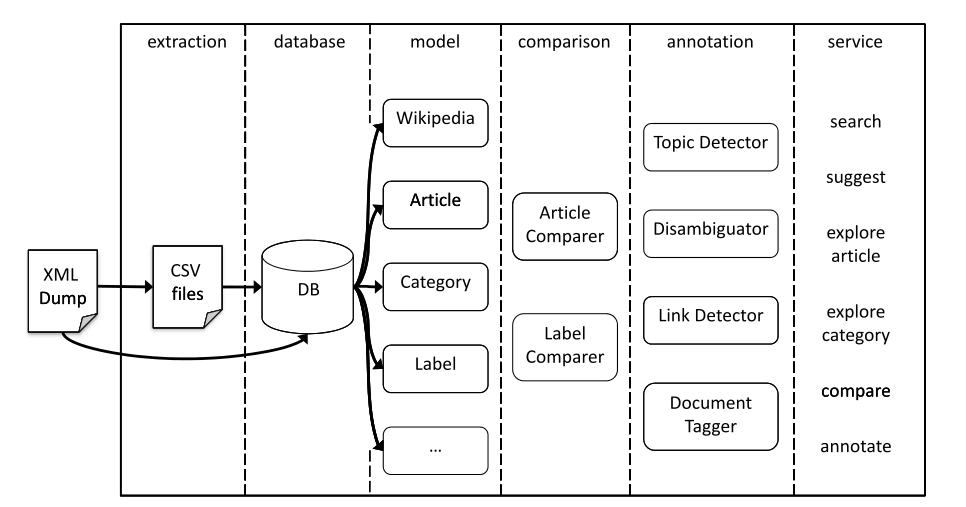
\includegraphics[scale=0.4]{img/wikipediaminer}
\caption{Wikipedia Miner architektúra (forrás: Artificial Intelligence, Wikipedia and Semi-Structured Resources \cite{aijournal})}
\label{fig:wikipediaminer}
\end{figure}

A rendszer áttekintő architektúráját mutatja be a \ref{fig:wikipediaminer}.~ábra. A rendszer belépési pontjára érkezik egy nagy méretű XML formátumú fájl, mely a Wikipédia hivatalos API-ján keresztül lett letöltve és tartalmazza a naprakész Wikipédia teljes állományát.

Az \textit{extraction} package funkciója, hogy kinyerjen az XML forrásból egy összegzett tartalmat. Az adatkinyerési folyamat használja a nagy méretű XML fájl feldolgozásához a Hadoop és MapReduce technológiákat, valamint a Google GFS fájlrendszerét. Az adatok kinyerése tehát elosztott rendszeren történik, a 27 GB méretű teljes angol Wikipédia feldolgozása a mérések szerint egy 2 magos, 2,66 GHz órajelű processzorral és 4 GB memóriával rendelkező 30 gépből álló clusternek 2,5 órájába telik.

A Wikipédia kivonatolása után a teljes XML fájl és az összegzett tartalmak is bekerülnek a \textit{database} package adatbázisába. Adatbázisként Berkeley DB Java Edition-t használnak, mellyel akár egy teljes adatbázist is a memóriában lehet tartani, ezzel nagyon gyors lekérdezhetőséget elérve.

A Wikipedia Miner keretrendszert használók a tartalmakhoz a \textit{model} package absztrakciós felületen keresztül férhetnek hozzá, mely becsomagolja a kinyert információkat és jól dokumentált osztályok formájában teszi közzé (mint például: \texttt{Wikpedia}, \texttt{Article}, \texttt{Category}).

A további csomagok (\textit{comparison} és \textit{annotation}) már a felhasználók számára használható szemantikus tartalom kezelését segítő eszközök, a \textit{service} package-ben pedig konkrét szolgáltatások találhatóak, melyeket felhasználhatnak a fejlesztők, illetve kiegészíthetik őket.

% section wikipediaminer (end)

\section{Tanulságok}
\label{sec:conclusion}

Amint látható a fentebb leírt Wikipédiát felhasználó eszközök szinte mind kizárólag a Wikipédia egy korábban letöltött változatán (dump) alapulnak, mely módszernek több hátránya is van. A letöltött tudásbázis mérete rendkívül nagy, így azt kezelni nehézkes, feldolgozási ideje rendkívül hosszú (a Wikipedia Processor feldolgozási ideje például körülbelül 43,5 óra). A hosszú feldolgozási idő nem mindig engedhető meg, ráadásul amíg nincs feldolgozott forrás, a rendszer sem működőképes. Újabb dump letöltésekor kezdhető előlről a feldolgozás, így többször is megakaszthatja ez a folyamat a rendszer működését, a rendelkezésre állási időt csökkentve.

A másik megoldás, melyet a Wikipedia Miner (\ref{sec:wikipediaminer}.~alfejezet) is demonstrál a Wikipédia folyamatos \textit{on-the-fly} feldolgozása. Míg az előző módszer figyelmen hagyja a közösségi tudásbázisok fő erejét, hogy rendkívül dinamikusan fejlődnek, az on-the-fly megoldás kihasználja azt, és mindig a friss adatokkal dolgozik.

További fontos megállapítások, hogy egyik rendszer sem elég flexibilis: futásidőben új komponens beépítése egyáltalán nem lehetséges, nem lehet a feldolgozólánchoz új elemet (kutatást végző modult) illeszteni, szerkezetük szinte mindegyiknek rendkívül statikus és csak arra a célra használhatóak konkrétan, amilyen speciális feladat ellátására kitalálták. Ebből adódóan rendkívül specifikusak és bonyolultak, így újabb kutatások indítása eredményeiket felhasználva nehézkes.

A szoftverek bármely módosítása újrafordítást, rendszerleállást eredményez, ami egy aktívan használt program számára nagy kiesést jelenthet. On-the-fly feldolgozásnál a rendszer leállása kihagyott, nem feldolgozott információkkal jár, így a tudásbázis töredezetté válhat. Ezen okok miatt szükséges egy olyan megoldás, mellyel a rendszer sokkal flexibilisebbé tehető és a fenti problémák áthidalhatóvá válnak.

% section conclusion (end)

% chapter related_work (end)
\chapter{Az OSGi keretrendszerről}
\label{cha:osgi}

Az OSGi Alliance \cite{osgi} által fejlesztett OSGi (\textit{Open Services Gateway initiative}) egy Java nyelvű, dinamikus, szolgáltatás orientált komponens modell és keretrendszer, mellyel kiterjeszthető az alap Java nyelven készült programok funkcionalitása. Használatával elérhető válik egy komponens alapú fejlesztés, ahol alkalmazásokat (illetve komponenseket) távolról elérve telepíthetjük, elindíthatjuk, leállíthatjuk, frissíthetjük, vagy törölhetjük anélkül, hogy a teljes alkalmazást leállítanánk és újra elindítanánk. A standard Java-val készült alkalmazásoknál ez egy fontos hiányosság, hiszen az információs rendszerek sok területén nem engedhetőek meg akár a pillanatnyi leállások sem. A flexibilitás és újrafelhasználhatóság követelményeknek tehát nagyon jól megfelel az OSGi keretrendszer, ezért is esett rá a választás.

\section{Bundle}
\label{sec:bundle}

Az OSGi technológiát \cite{osgiintro} használó alkalmazások kisebb komponensekre (az OSGI terminológiát használva csomagokra, azaz \textit{bundle}-ökre) vannak bontva. Ezen csomagok elkészíthetőek, lefordíthatóak, telepíthetőek egymástól függetlenül, életciklusukat maga az OSGi keretrendszer felügyeli. A bundle-ök gyakorlatilag nem mások, mint a jól ismert JAR fájlok (Java osztályok, és egyéb erőforrások), azzal a különbséggel, hogy a leíró manifest állományban a szabvány által kiterjesztett módon további fejlécek találhatóak meg. Példát látunk manifest állományra a \ref{lst:manifest}.~kódrészletben.

A manifest állomány elemei:

\begin{description}
	\item[Bundle-Name] az elkészített bundle emberek számára olvasható neve
	\item[Bundle-SymbolicName] Java package név, ez azonosítja a bundle-t (az egyetlen kötelező elem)
	\item[Bundle-Description] a bundle hosszabb szöveges leírása
	\item[Bundle-ManifestVersion] a bundle által használt OSGi változat verziószáma
	\item[Bundle-Version] a bundle verziószáma
	\item[Bundle-Activator] BundleActivator interfészt implementáló bundle-ben lévő osztály, mely a bundle telepítése után elindul
	\item[Export-Package] más bundle-ök számára elérhetővé tett saját csomagok és verziószámaik listája
	\item[Import-Package] a bundle fordításához és futtatásához szükséges külső csomagok listája
	\item[Private-Package] olyan saját csomagok, amelyeket nem teszünk elérhetővé más bundle-ök számára
\end{description}

\begin{lstlisting}[label={lst:manifest}, caption=MANIFEST.MF,breaklines=true]
Bundle-Name: Hello World
Bundle-SymbolicName: org.available.helloworld
Bundle-Description: A Hello World bundle
Bundle-ManifestVersion: 2
Bundle-Version: 1.0.0
Bundle-Activator: org.available.helloworld.Activator
Export-Package: org.available.helloworld;version="1.0.0"
Import-Package: org.osgi.framework;version="1.3.0"
Private-Package: org.notavailable.helloworld
\end{lstlisting}

% section bundle (end)

A bundle-ök egy OSGi példányon belül, azonos JVM-ben futnak. Ennek vannak előnyei (teljesítmény növekedés, kisebb erőforráshasználat, interprocess kommunikációt nem szükséges használni), de hátrányai is (hozzáférési problémák), melyeket az OSGi úgy old meg, hogy minden bundle-höz saját classloader-t rendel.

\section{Service, Service Registry}
\label{sec:service}

A bundle-ök kiajánlhatnak szolgáltatásokat (\textit{service}), melyekre más bundle-ök feliratkozhatnak. Az OSGi specifikáció szerint a szolgáltatások normál Java objektumok, melyek egy adott interfészt implementálva lettek beregisztrálva az OSGi \textit{Service Registry} moduljába.

A Service Registry segítségével tudnak tehát a bundle-ök kiajánlani szolgáltatásokat, rajtuk keresztül tudják lekérdezni az elérhető szolgáltatásokat. Ha egy bundle-nek szüksége van egy másik bundle által kiajánlott szolgáltatásra, akkor az OSGi keretrendszer megteremti közöttük a kapcsolatot és a kért szolgáltatást használhatja az adott bundle.

% section service (end)

\section{Életciklus}
\label{sec:lifecycle}

\begin{figure}[htb]
\centering
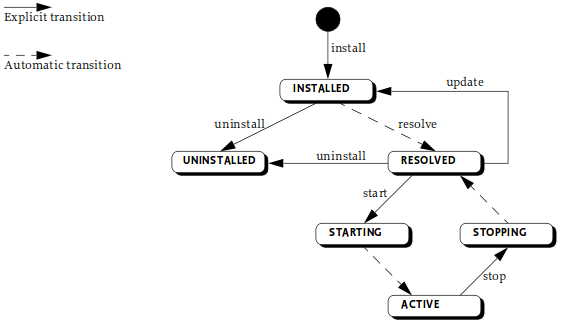
\includegraphics[scale=0.5]{img/bundle_lifecycle}
\caption{Bundle életciklus (forrás: OSGi Service Platform Release 2 \cite{osgi})}
\label{fig:bundle_lifecycle}
\end{figure}

\begin{table}[htb]
\begin{center}
\begin{tabular}{|c|c|}
\hline
\textbf{Állapot neve} & \textbf{Leírás} \\
\hline
\hline
INSTALLED   & A bundle sikeres telepítve lett. \\
\hline
RESOLVED    & A bundle-nek minden függősége ki lett elégítve. Kész az elindításra, vagy már le lett állítva. \\
\hline
STARTING    & A bundle el lett indítva, de még nincs aktiválva, .start() metódus még nem tért vissza. \\
\hline
ACTIVE      & A bundle aktiválva lett és aktív. \\
\hline
STOPPING    & A bundle le lett állítva, .stop() metódus még nem tért vissza. \\
\hline
UNINSTALLED & A bundle el lett távolítva, ez az életciklus végállapota. \\
\hline
\end{tabular}
\end{center}
\caption{\label{tab:lifecycle_states} Bundle életciklus állapotai}
\end{table}

Az OSGi keretrendszer dinamikusságát a \textit{Life-cycle} (életciklus) modul szolgáltatja, mely által a bundle-öket futásidőben lehet telepíteni, elindítani, leállítani, frissíteni, eltávolítani más hagyományos alkalmazásokkal ellentétben. A bundle-ök futtatása előtt megvizsgálja a keretrendszer a csomag futás idejű függőségeit, és ha olyan kielégítetlen függőségeket talál, melyek szükségesek a bundle futtatásához, akkor nem indítja el a komponenst.

Egy bundle életciklusának állapotai megfigyelhetőek a \ref{fig:bundle_lifecycle}.~ábrán, valamint az állapotok leírása a \ref{tab:lifecycle_states}.~táblázatban látható.

% section lifecycle (end)

% chapter osgi (end)
\chapter{Tervezés}
\label{cha:design}

Ahogy a \ref{cha:osgi}.~fejezetben is láttuk az OSGi keretrendszer megfelel a kiírásban specifikált szoftver által támasztott követelményeknek, felhasználásával a rendszer kellően flexibilis lesz. Az \ref{cha:related_work}.~fejezetben levont tanulságok alapján érdemes megtervezni a rendszert, illetve az ott említett Wikipédia Miner architektúráját fel lehet használni a tervezés során, az alapvető komponensek meghatározásában segíthet.

Első lépésként meghatároztam a leendő rendszer komponenseit (\ref{fig:componentdiagram}.~ábra), mely képes folyamatosan működve a Wikipédia tartalmát rendszerezett formában eltárolni és azt később a rá épülő alkalmazások számára elérhetővé tenni. Mivel a rendszer első indításakor az adatbázisban még semmilyen adatok nem találhatóak, és a Wikipédia frissülő cikkeinek követésével, csak az aktuális változások kerülnek be az adatbázisba, a rendszer indításakor már a Wikipédián korábban közzétett cikkek nem kerülnek be a felépített tudásbázisba. Ezt a problémát úgy lehet a legegyszerűbben megoldani, hogy az on-the-fly feldolgozás mellett a statikus dumpból való adatok importálását is lehetővé tesszük. Ezzel kombináljuk a \ref{cha:related_work}.~fejezetben megismert alkalmazások előnyét a követelményekben meghatározottakkal, így egy sokkal erősebb eszköz állítható elő.

\begin{figure}[htp]
\centering
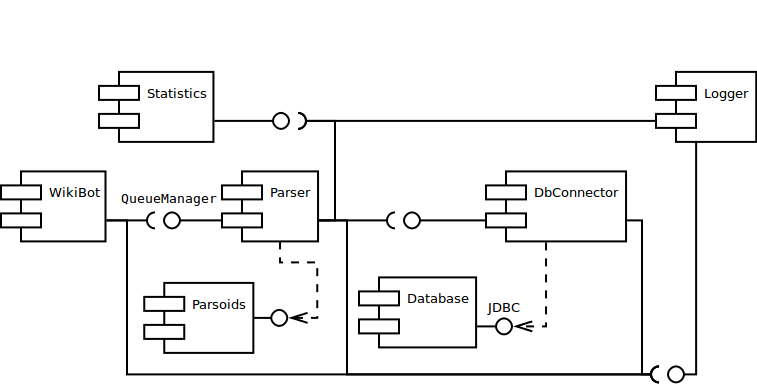
\includegraphics[scale=0.5]{img/componentdiagram}
\caption{Az alkalmazás tervezett komponensei}
\label{fig:componentdiagram}
\end{figure}

A követelményekből következően szükségszerűen meghatározott komponenseken túl az alkalmazás minőségének javítása érdekében érdemes a komponensek felügyelhetőségét is biztosítani. Ezáltal az alkalmazás működéséből részletesebb adatok is megfigyelhetővé válnak azon kívül, hogy működik vagy sem a rendszer, illetve a funkcionalitás tesztelése és a teljesítménymérés is sokkal egyszerűbb lesz. A felügyelhetőséget naplózás és különféle metrikák segítségével terveztem lehetővé tenni.

Miután a különálló komponenseket meghatároztam, megkezdődhetett sorban az egyes komponensek megtervezése. Minden komponenst a komponensalapú fejlesztésnek megfelelően egyesével, mint különálló programokat lehetett megtervezni és implementálni. A következőkben bemutatom az egyes komponensek szerepét, alapvető működését és a tervezésük lépéseit.

\section{WikiBot bundle}
\label{sec:wikibotbundle}

Az adatok on-the-fly feldolgozásáért felelős ez a komponens. Ezt a tulajdonságot a frissülő cikkek megszerzésének módjával fogom biztosítani. Az adatok könnyű kezelése miatt minden cikknek egy reprezentációját is ki kell alakítani a programban, amelyet tovább kell adni a következő komponensek számára, további feldolgozás céljából. Ezek alapján meghatározott use-case-ek láthatóak a \ref{fig:usecase_wikiBot}.~ábrán.

\begin{figure}[htp]
\centering
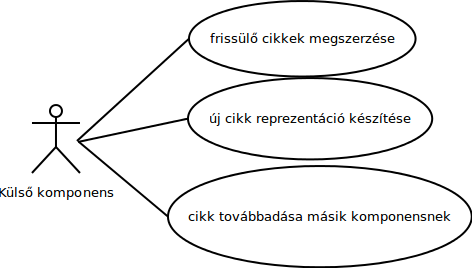
\includegraphics[scale=0.6]{img/usecase_wikiBot}
\caption{A WikiBot komponens használati esetei}
\label{fig:usecase_wikiBot}
\end{figure}

Megtervezését egy rövidebb előkutatás előzte meg, mely során keresni kellett valamilyen lehetőséget, amelynek segítségével folyamatosan értesülhet az alkalmazás, ha egy új Wikipédia cikk jelenik meg, vagy frissítenek egyet a hivatalos oldalon. A legegyszerűbb megoldásnak végül a hivatalos, Wikipédia által üzemeltett IRC csatorna tűnt, ahol folyamatosan publikálják az oldalon frissülő cikkeket.

\begin{figure}[htp]
\centering
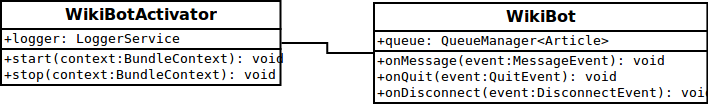
\includegraphics[scale=0.55]{img/class_wikiBot}
\caption{A tervezett WikiBot osztálydiagramja}
\label{fig:class_wikiBot}
\end{figure}

A tervezett komponens tehát egy IRC Bot kliens lesz, amely a fent említett IRC csatornára lesz feliratkozva. A tervezésnél figyelni kellett arra, hogy miután megszerzi az új cikk szükséges adatait, azokat azonnal tovább kell adnia a következő komponensnek. Más teendőket nem végezhet, működését nem szabad hosszú távon feltartani, mert a gyorsan frissülő cikkek miatt elvesznek az IRC csatorna által küldött információk, míg a komponens mással foglalkozik.

A komponens két osztályból fog állni, az egyik egy OSGi BundleActivator implementáció (\texttt{WikiBotActivator} osztály), mely menedzseli a komponens indulását, leállítását, a másik pedig a Wikipédia IRC csatornájával való kommunikációt kezeli (\texttt{WikiBot}).

A tervezett működés szerint a rendszer a \texttt{WikiBotActivator} elindulásával kezdődik, melyet az OSGi keretrendszer példányosít számunkra, majd elindítja azt. A lehető leggyorsabb működés úgy érhető el, hogy ne tartsuk fel a komponens működését, ha az új cikk megszerzett adatait eltároljuk egy átmeneti tárolóban (\texttt{QueueManager} osztály). Ez a queue, ahogy a \ref{fig:componentdiagram}.~ábrán is látható a Parser komponens egy kiajánlott OSGi szolgáltatása. A \texttt{QueueManager} osztály bemutatása a \ref{sec:parserbundle} alfejezetben folytatódik. A kiajánlott queue referenciáját az OSGi \texttt{BundleContext}-en keresztül lehet majd megszerezni.

Továbbiakban a \texttt{WikiBot} belép a Wikipédia egyik IRC szobájába, ahol az angol nyelvű cikkeket teszik közzé. Az implementált IRC Bot-ban egy eseménykezelőt kell megvalósítani (\texttt{.onMessage()} metódus), ami akkor hívódik meg, ha egy új üzenet érkezik az IRC szobába. Egy példa üzenet figyelhető meg a \ref{lst:ircexample}.~kódrészletben.

\begin{lstlisting}[label={lst:ircexample}, caption=Példa üzenet az angol nyelvű Wikipédia IRC csatornájából,breaklines=true]
(11.16.43) rc-pmtpa: [[History of Vietnam]]  http://en.wikipedia.org/w/index.php?diff=580135314&oldid=580104406 * 124.170.231.126 * (+95) 
\end{lstlisting}

Minden egyes beérkezett üzenet alapján egy új cikk reprezentációt (\texttt{Article} osztály) hoz létre, mely később végig fog haladni a teljes feldolgozóláncon. A szükséges adatok a cikk címe, mely dupla szögletes zárójelek között található, valamint az új cikk verziószáma, mely az üzenetben található link \texttt{diff} GET paraméterében található. Végül az összeállított cikket a korábban megszerzett \texttt{QueueManager}-ben helyezi el.

Az alapvető követelményeken felül a megfigyelhetőséget is érdemes biztosítani, amelyet a \texttt{WikiBot} komponensnél naplózással oldottam meg. A \texttt{WikiBotActivator} indulásakor a \texttt{Logger} komponens (\ref{sec:loggerbundle}.~alfejezet) referenciáját is megszerzi, melyet naplózásra használhat.

% section wikibotbundle (end)

\section{Parser bundle}
\label{sec:parserbundle}

Ebben a komponensben kell lennie valamilyen tároló elemnek, egyfajta queue megoldásnak, melynek szükségessét az előző \ref{sec:wikibotbundle}.~alfejezetben fejtettem ki. Ennek a queue megoldásnak szálbiztosnak kell lennie, hiszen egyszerre fog a WikiBot és a Parser komponens dolgozni vele, ezenkívül a tárolónak blokkolnia is kell beszúrást, ha már túl sok elem van benne. A módosult, vagy újonnan létrehozott cikkek szövegét meg kell szereznie a komponensnek, majd azt át kell alakítania egy meghatározott formátumra. Végül a cikket tovább kell adnia egy másik komponensnek eltárolás céljából. Ezek alapján készíthető el a a use-case diagram (\ref{fig:usecase_parser}.~ábra).

\begin{figure}[htp]
\centering
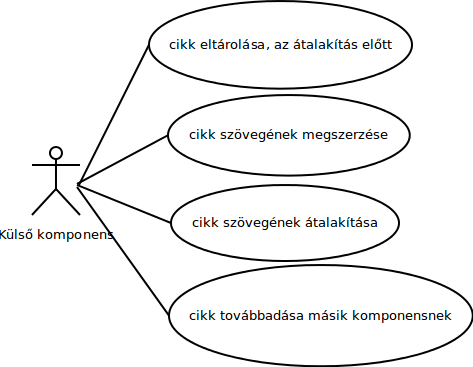
\includegraphics[scale=0.6]{img/usecase_parser}
\caption{A Parser komponens használati esetei}
\label{fig:usecase_parser}
\end{figure}

Ahhoz, hogy egy másik komponens el tudjon tárolni a Parser-ben valamit, létre kell hozni a Parser komponensben egy szolgáltatást (OSGi service), amelyen keresztül a kommunikáció megtörténhet. Ez az szolgáltatás egyben az egész program mozgatórugója is, hiszen a további use-case-ekben található funkciókat akkor tudjuk végrehajtani, ha legalább egy cikk már el lett tárolva.

Ennél a résznél használtam az \textit{Observer} tervezési mintát \cite{designpatterns}: a \texttt{QueueManager} osztály \texttt{Observable} lett, míg egy \texttt{Observer}-ből származó \texttt{WikiObserver} kezelte a tárolóba került új elemeket (\ref{fig:class_parser}.~ábra).

\begin{figure}[htp]
\centering
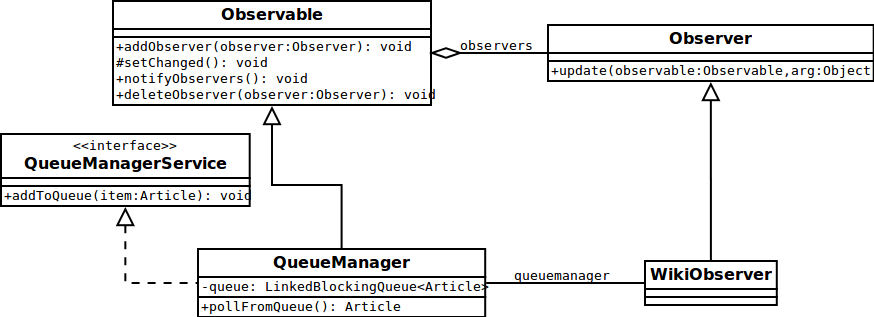
\includegraphics[scale=0.5]{img/class_parser}
\caption{Observer minta használata a Parser komponensben}
\label{fig:class_parser}
\end{figure}

Az Observer tervezési mintának köszönhetően, ha új elem kerül a queue-ba, akkor arról a \texttt{WikiObserver} értesülni fog. Mivel a cikkek feldolgozása jelentős időt vehet igénybe, azt mindenképpen külön szálakon kell megtenni. Ezt a problémát a \textit{Threadpool} tervezési mintával oldottam meg \cite{javaconcurrencyinpractice}. A \texttt{WikiObserver}-nek (\ref{fig:class_parser2}.~ábra) van egy \texttt{ThreadPool} példánya, és ha értesül a queue frissüléséről, egy új feladatot fog a \texttt{ThreadPool}-hoz hozzáadni. A ThreadPool mintának megfelelően minden feladat (\texttt{WikiWorker}) külön szálon fut. 

\begin{figure}[htp]
\centering
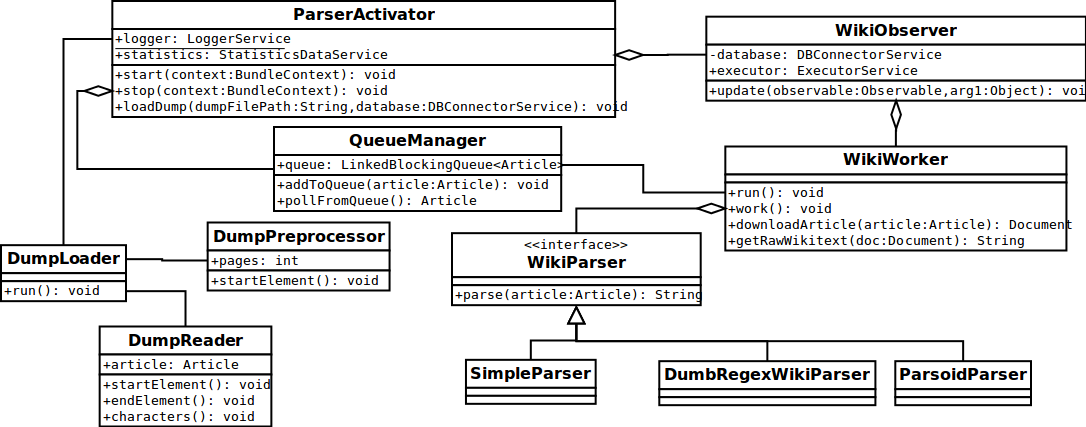
\includegraphics[scale=0.55]{img/class_parser2}
\caption{A Parser komponens osztálydiagramja}
\label{fig:class_parser2}
\end{figure}

Ebben a fázisban első lépésben először letöltődnek a hivatalos Wikipédia API-n keresztül a cikkek tartalmai. A Wikipédia a felhasználók számára könnyebben szerkeszthető \textit{Wikitext} formátumban teszi elérhetővé a cikkek tartalmait. A Wikitext egy egyszerű, könnyen használható jelölőnyelv, mely egyértelműen leképezhető a HTML formátumra, így könnyen készíthetőek vele webes tartalmak.

Azonban ez a Wikitext formátum kevésbé jól feldolgozható, mint például a HTML formátum, így a cikkek szövegét HTML formába célszerű alakítani. A második fázisban tehát ez az átalakítás történik meg, ha nem volt még újabb verziójú változat az adott cikkből az adatbázisban. Ehhez ún. parser-eket lehet használni, melyből három felcserélhető, különböző előnyökkel és hátrányokkal rendelkező változat is került a feldolgozóláncba.

\begin{itemize}
	\item Sztakipedia parser \cite{sztakipediaparser}: Könnyen testreszabható és általános célú program, mely a MediaWiki Wikitext formátumról tud HTML formátumra átalakítani. Oláh Tibor BME mérnök informatikus hallgató 2011. évi gyakornoki munkája az MTA SZTAKI-ban. Ez a program egy könnyen kiterjeszthető \textit{Visitor} tervezési mintára alapuló szoftver, mely önálló csomagként is használható a jól felépített API-nak köszönhetően. Használata nagyon egyszerű, használható kimenetet állít elő és sebesség szempontjából is jól teljesít, viszont nagyon nagy méretű fájloknál, például egy teljes Wikipédia dump feldolgozásánál rendkívül sok memóriát használ. Ennek a tulajdonságnak köszönhetően, csak on-the-fly feldolgozás során használható eredményesen ez a parser.
	
	\item DumbRegexWikiParser parser: A végletekig leegyszerűsített MediaWiki Wikitext átalakító Héder Mihály 2011. évi munkája, mely egy SAX parser implementáció. Az állapotgépes Wikitext feldolgozásnak köszönhetően nem fogyaszt annyi memóriát, mint a Sztakipedia parser, sebesség szempontjából még gyorsabb is az előzőnél, viszont kevésbé használható kimenetet produkál.
	
	\item Parsoid parser: Ez az átalakító a WikiMedia Alapítvány által, 2011 óta fejlesztett és használt szoftver, mely a Wikitext egy ekvivalens HTML / RDFa kimenetét készíti el, mely automatikus feldolgozásra rendkívül jól használható. Az RDFa szabványban meghatározott attribútumokkal kiegészített HTML kód, sokkal nagyobb jelentéstartalommal bír, mint az alap HTML dokumentum, így a szöveg sokkal jobb lesz további felhasználhatóság szempontjából. A Parsoid egy NodeJS-ben írt szoftver, így felhasználása Java nyelvű alkalmazásokban sokkal nehezebb, mint a korábbi parser megoldásoké, viszont kimenete a célnak leginkább megfelelő, így ez lett az ajánlott átalakító mechanizmus a feldolgozóláncban.
\end{itemize}

Végül a cikk feldolgozásának utolsó, harmadik fázisában eltárolódik a cikk a rendszer adatbázisában. Ebbe a fázisba akkor ér el a feldolgozás, ha nem volt újabb verziójú változat az adott cikkből még az adatbázisban. A verziók meghatározása a cikkek verziószáma alapján történik. Ha régebbi verziószámú cikk már volt az adatbázisban, akkor azt csak frissíteni kell, ellenkező esetben az adott cikknek még semmilyen változata nem létezik az adatbázisban, így azt újonnan kell beszúrni.

Ennél a komponensnél a  megfigyelhetőséget naplózással és különféle metrikák lekérdezhetőségével oldottam meg. A \texttt{ParserActivator} indulásakor a \texttt{Logger} komponens (\ref{sec:loggerbundle}.~alfejezet), és a \texttt{Statistics} komponens (\ref{sec:statisticsbundle}.~alfejezet) referenciáját is megszerzi.

\subsection{Wikipédia dump feldolgozás}
\label{sub:dumpprocessing}

A feldolgozólánc indulásakor, lehetőség van az éppen frissülő cikkek on-the-fly feldolgozásán és adatbázisba való eltárolásán túl a már korábban a Wikipédián elérhető cikkek eltárolására is, melynek forrása a havonta frissülő Wikipédia állománya, amit XML formátumban tesznek elérhetővé.

A dump feldolgozása nagyon hasonlít az on-the-fly feldolgozáshoz, szintén egy \texttt{WikiObserver} példány irányítja a feldolgozást és egy \texttt{QueueManager}-t használ a cikkek ideiglenes eltárolásához. A hatalmas méretű (2013. októberében 44 GB) XML fájl, melyben a Wikipédián olvasható cikkek vannak eltárolva, a feldolgozás során először egy előfeldolgozáson megy keresztül, ahol gyorsan néhány statisztikai adatot gyűjt a program az adatbázismentésről. Ilyen statisztikai adat például a dump-ban lévő cikkek száma, így követhető a feldolgozás állapota a tényleges beolvasás során. Ekkora méretű fájlt csak valamilyen állapotgép alapú megoldással lehet feldolgozni, ilyen például \textit{SAX Parser} (Simple API for XML). A parser a megszerzett cikket egy queue-ban tárolja el, ahonnan a \texttt{WikiObserver} kiszedi, annak szövegét átalakítja HTML formátumra és eltárolja az adatbázisban.

% subsection dumpprocessing (end)

% section parserbundle (end)

\section{DatabaseConnector bundle}
\label{sec:dbconnectorbundle}
    
Ebben a komponensben lesz az adatbázisban eltárolva a Parser komponens által feldolgozott minden cikk. Feladatai közé tartoznak tehát az adatbáziskezeléssel kapcsolatos műveletek elfedése más rétegek elől: cikkek eltárolása, frissítése, törlése és különböző szempontok alapján való keresés a cikkek között, azaz a CRUD műveletek (create, read, update, delete). A feldolgozóláncra alapuló további rétegek számára -- melyet külső fejlesztők (a rendszer felhasználói) készítenek -- ez a komponens egy csatlakozási pont, így kiajánlott szolgáltatását alacsonyabb és magasabb rétegben lévő komponensek is használhatják, az adatbázissal való kommunikáció teljesen el van fedve előlük.

\begin{figure}[htp]
\centering
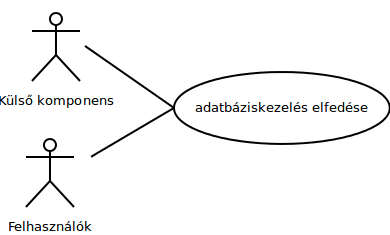
\includegraphics[scale=0.6]{img/usecase_dbconnector}
\caption{A DBConnector használati esetei}
\label{fig:usecase_dbconnector}
\end{figure}

A fenti use case-ek csak általánosan fogalmazzák meg a komponenssel kapcsolatos elvárásokat. Az egyes feldolgozóláncra alapuló komponensek további követelményeket is támaszthatnak a komponens iránt, például különböző szempontok alapján való keresés.

\begin{figure}[htp]
\centering
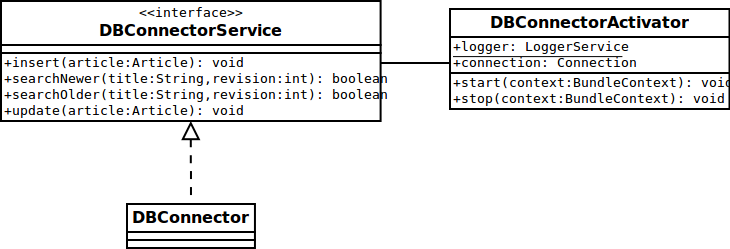
\includegraphics[scale=0.55]{img/class_dbconnector}
\caption{A DBConnector komponens osztálydiagramja}
\label{fig:}
\end{figure}

A komponens indulásakor (\texttt{DBConnectorActivator} osztály \texttt{.start()} metódusa), olyan állapotba hozza az adatbázist, hogy az később képessé váljon a fenti feladatokra, valamint egy OSGi szolgáltatást kell kiajánlani, amin keresztül a többi komponens kommunikálhat a DBConnector-ral.

% section dbconnectorbundle (end)

\section{Database}
\label{sec:db}

Az adatbázis komponens alapjául szolgáló adatbázis szoftver kiválasztását a WikiBot komponenshez hasonlóan egy rövidebb előkutatás előzte meg. Fő szempont volt, hogy nagy teljesítményű, gyors és lehetőleg az OSGi keretrendszerrel könnyen integrálható legyen a választott adatbázis megoldás. Két különböző adatbázis lehetőséget vizsgáltam meg, és a tapasztalatok alapján választottam ki a legmegfelelőbbet.

\begin{enumerate}
	\item Prevayler: Egy nagyon egyszerű és gyors adatbázis, melynek lényege, hogy minden objektumot egyszerű Java objektumokként (POJO) tartsunk a memóriában, és a tranzakciókat naplózzuk, az adatbázis pedig a használó programba beágyazottan fut. A tárolandó objektumokra egyetlen megkötés, hogy implementálják a \texttt{Serializable} interfészt, és a műveleteket is szerializálható objektumok reprezentálják. A műveleteket a Prevayler naplózza, és időnként teljes mentést (\textit{snapshot}) készít az adatbázisról, így egy rollback esetén a snapshot-ot visszaállítja és lefuttatja még a szükséges tranzakciókat.
	
Felépítéséből adódóan sokkal gyorsabb mint bármelyik RDBMS, viszont OSGi környezetben a használata egyelőre nem megoldott. A probléma oka, hogy minden OSGi komponensnek saját classloader-e van, így osztályok dinamikus betöltése, például szerializációval nem lehetséges az OSGi programokban \cite{hall04osgi}. A megoldás lehetne új \texttt{BundleClassLoader} implementálása, azonban ez a Prevayler használatának egyszerűségét rontaná el, így inkább másik megoldást választottam.

    \item H2DB: Az összegyűjtött tapasztalatok alapján arra jutottam, hogy OSGi környezetben kevésbé érdemes beágyazott adatbázist választani, ha több komponens között is meg kell oldani a kommunikációt, hiszen belső működésüket tekintve ezen adatbázisok szinte mindig használnak valamilyen szerializációs eljárást.

    A H2DB egy objektum relációs adatbázis, mely tud beágyazott és kliens-szerver módban is működni. A készítők teljesítménytesztjei alapján gyorsabb a legtöbb népszerű adatbáziskezelőnél (HSQLDB, Derby, MySQL, PostgreSQL), valamint tervezésekor megpróbálták a HSQLDB és a Derby adatbáziskezelők előnyeit is egyesíteni benne.

A H2DB további előnyei még, hogy nem szükséges telepíteni, teljes egészében Java nyelven íródott és például Java nyelvű tárolt eljárásokkal is kiegészíthetjük funkcióit. Az eddig felsorolt pozitív tulajdonságok miatt esett a választásom a H2DB-re, bár igaz, hogy beágyazott módban OSGi-al nem használható effektíven, csak úgy, mint a Prevayler. A H2DB szerver módban is használható, így JDBC adatbázishozzáférési API-val lehet kapcsolódni hozzá. A szerver módban való futtatás előnye, hogy sokkal kisebb a csatolás az adatbázissal, így például a DBConnector komponensben, ha a JDBC API-t használjuk, az adatbázis könnyen lecserélhető a rendszerben másik adatbázis megoldásra.

\end{enumerate}

\begin{figure}[htp]
\centering
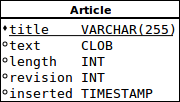
\includegraphics[scale=0.8]{img/database_article}
\caption{A tervezett adatbázis Article táblája}
\label{fig:database_article}
\end{figure}

Az adatbázis kiválasztása után, az adatbázis tábláinak megtervezése következett. Az egyszerű specifikáció miatt egyed kapcsolat diagram rajzolására nincs szükség, hiszen egyetlen egyed van az adatbázisban, mely a cikk reprezentációja (\texttt{Article}). A Wikipediában minden cikket annak címe azonosítja (\ref{fig:database_article}.~ábra), nem lehet két azonos című, de különböző cikk. Így elsődleges kulcs a cím (title) lesz, további szükséges attribútumok a szöveg (text), szöveg hossza (length), szöveg verziószáma (revision), illetve a beillesztés dátuma (inserted).

A rendszerben természetesen további adatbázisok, táblák is lehetnek, amelyeket a kutatómodulok hozhatnak létre. Ezek a kutatómodulok a rendszer által előfeldolgozott Article példányokat elemzik tovább. A DatabaseConnector komponens könnyen kiegészíthető, hogy a kutatómodulok igényeit teljesítse, azonban ez már nem az én feladatom volt.

% section db (end)

\section{Logger bundle}
\label{sec:loggerbundle}

Ha a rendszer állapotait meg akarjuk figyelni, illetve szeretnénk, ha jelezné a hibákat, mindenképpen érdemes az alkalmazást felügyeletre tervezni. Az egyik ilyen lehetőség a naplózás, mely ennek a komponensnek a fő feladata (\ref{fig:usecase_logger}.~ábra).

\begin{figure}[htp]
\centering
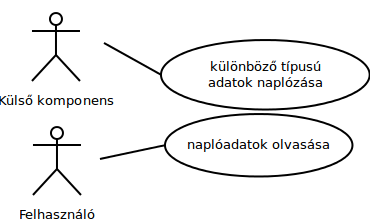
\includegraphics[scale=0.6]{img/usecase_logger}
\caption{A Logger komponens használati esetei}
\label{fig:usecase_logger}
\end{figure}

Első lépésben meg kell tervezni a rendszer felügyeleti modelljét, mely egy állapotgép formájában ábrázolható a rendszer fontosabb állapotaival. Az állapotgép átmenetei események, az átmenetek feltételei hibalehetőségek, a tranzakciók pedig naplózást jelentenek, a használt jelölés:

\begin{equation}
	esem\acute{e}ny(argumentum) [felt\acute{e}tel] / tranzakci\acute{o}
\end{equation}

Naplózás során a rendszer eseményeit több kategóriába soroltam be súlyosság és következmények szempontjából, ezek láthatóak a \ref{tab:loglevels}.~táblázatban.

\begin{table}[htb]
\begin{center}
\begin{tabular}{|c|l|}
\hline
\multicolumn{1}{|c|}{\textbf{naplózási szint}} & \multicolumn{1}{|c|}{\textbf{rövid leírás}} \\ \hline \hline
FATAL & Súlyos hiba, amely a rendszer leállásához vezet. \\ \hline
ERROR & Súlyos hiba, azonban a rendszer működése nem feltétlenül áll meg. \\ \hline
WARN  & Esetlegesen káros hatással bíró esemény. \\ \hline
INFO  & Magasszintű információ a rendszer állapotáról. \\ \hline
DEBUG & Részletes információk a rendszer állapotáról, hibakereséshez használható. \\ \hline
TRACE & Legrészletesebb információk a rendszer állapotairól. \\
\hline
\end{tabular}
\end{center}
\caption{\label{tab:loglevels} A naplózás szintjei}
\end{table}

A fent meghatározott naplózási szinteknek megfelelő naplózási eljárásokat teljesítő komponens egy OSGi szolgáltatás lesz, mely képes a naplózást a követelményeknek megfelelően elvégezni (\ref{fig:class_logger}.~ábra).

\begin{figure}[htp]
\centering
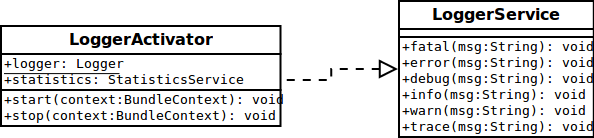
\includegraphics[scale=0.55]{img/class_logger}
\caption{A Logger komponens osztálydiagramja}
\label{fig:class_logger}
\end{figure}

% TODO: felügyeleti modellek aktualizálása

% section loggerbundle (end)

\section{Statistics bundle}
\label{sec:statisticsbundle}

Az alkalmazás felügyeletének másik lehetőségével meghatározott metrikák lekérdezésére és vizsgálatára van lehetőség. A többi komponens állapotait ennek a komponensnek a segítségével teheti elérhetővé, így a rendszer által végzett feladatról készített statisztikák megfigyelésére is van lehetősége a felhasználóknak (\ref{fig:usecase_statistics}.~ábra).

\begin{figure}[htp]
\centering
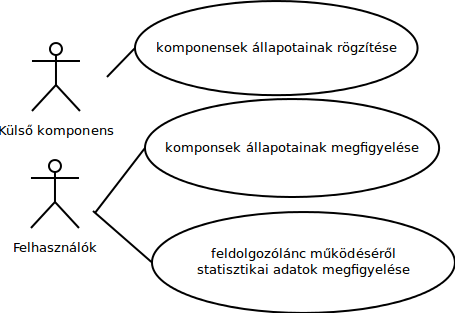
\includegraphics[scale=0.6]{img/usecase_statistics}
\caption{A Statistics komponens használati esetei}
\label{fig:usecase_statistics}
\end{figure} 

A feldolgozólánc működését átvizsgálva meghatároztam és kiválasztottam megfigyelés céljából a rendszer állapotának szempontjából fontos mérőszámokat (\ref{tab:metrics}.~táblázat).

\begin{table}[hbt]
\begin{center}
\begin{tabular}{|L{2.6cm}|L{4.5cm}|L{2cm}|L{4.7cm}|}
\hline
\textbf{metrika neve} & \textbf{metrika leírása} & \textbf{metrika mértékegy-sége} & \textbf{metrika számításának módja} \\ \hline \hline
eltárolt cikkek száma & ennyi cikk van az adatbázisban & darab & frissített cikkek száma + újonnan beillesztett cikkek száma \\ \hline
frissített cikkek száma & korábban már az adatbázisban szereplő, frissített cikkek száma & darab & ha kisebb verziószámú azonos című cikk szerepel az adatbázisban, akkor eggyel nő a száma \\ \hline
újonnan beillesztett cikkek száma & korábban még az adatbázisban nem szereplő cikkek száma & darab & ha még nem volt az adatbázisban az adott című cikk akkor eggyel nő a száma \\ \hline
nem feldolgozott cikkek száma & ennyi cikket nem dolgoztunk fel, mert újabb változat van az adatbázisban & darab & minden esetben mikor újabb verziójú cikket dolgoz fel a száma nő eggyel \\ \hline
hibák száma & FATAL, ERROR, WARN, DEBUG, INFO, TRACE üzenetek száma a naplóban & darab & log üzenet írása esetén a statisztikák száma is nő \\ \hline
queue hossza & QueueManager által karbantartott queue-ban lévő elemek száma & darab & QueueManager-be íráskor értéke nő eggyel, elem kivételekor csökken eggyel \\ \hline
feldolgozás sebessége & ennyi cikket dolgoz fel 1 perc alatt a feldolgozólánc & cikk/perc & 1 percenként elmentett cikkek számából kivonja az előző elmentett értéket \\ \hline
dolgozóparserek száma & adott nevű observerben ennyi parser dolgozik & százalék & dolgozó parserek száma / az összes elérhető parserek számával \\ \hline
dump feldolgozás állapota & ekkora százaléka lett beolvasva a dump-nak & százalék & beolvasott cikkek száma / összes cikk a dump-ban \\
\hline
\end{tabular}
\end{center}
\caption{\label{tab:metrics} A Statistics komponens által megfigyelhető metrikák}
\end{table}

Az eddigi követelmények alapján úgy tűnhet, hogy a legjobb választás a JMX (Java Management Extensions) technológia lenne a feladatra, azonban több szempont alapján sem ezt választottam. Bár később a rendszer valamilyen szintű menedzselése szükségessé válhat, mégis OSGi környezetben nem biztos, hogy a JMX a legjobb megoldás. Egyrészt a JMX nem építhető be a már korábban említett OSGi tulajdonságok miatt a rendszerbe, így egy másik implementációt a MOSGi-t (Managed OSGi) kellene használni; másrészt a MOSGi egy sokkal bonyolultabb architektúrát használ és a felhasználók számára sem annyira egyszerű a kezelése.

\begin{figure}[htp]
\centering
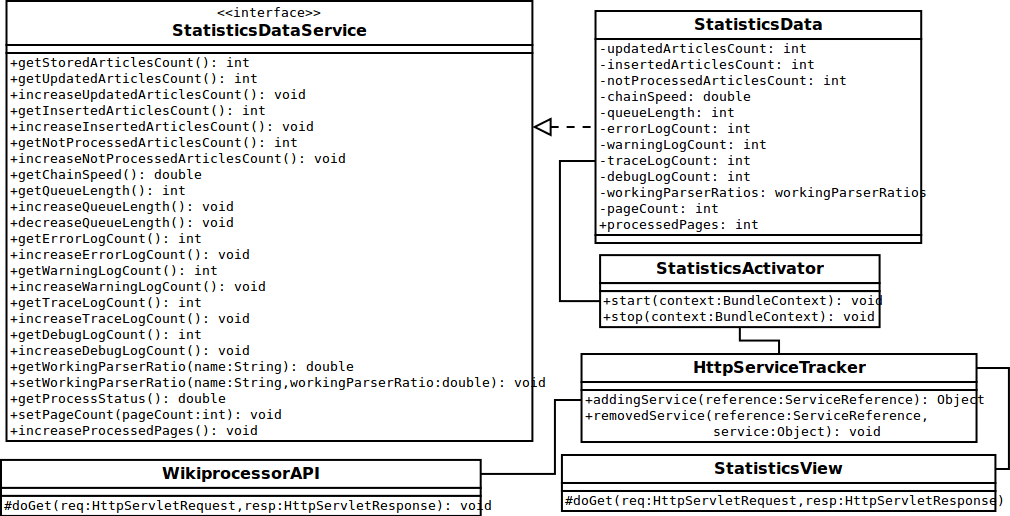
\includegraphics[scale=0.45]{img/class_statistics}
\caption{A Statistics komponens osztálydiagramja}
\label{fig:class_statistics}
\end{figure}

A fent felsorolt indokok alapján döntöttem saját menedzselő komponens fejlesztése mellett, mely egy sokkal egyszerűbb architektúrát követ, és nagyon könnyen kiegészíthető. A menedzser komponens egy OSGi szolgáltatásból áll (\texttt{StatisticsDataService} a \ref{fig:class_statistics}.~ábrán), melybe a többi komponens rögzítheti az állapotait, illetve két servlet segítségével tud kapcsolatba lépni a felhasználókkal, melyek közül az egyik JSON formátumban elérhetővé teszi a statisztikai adatokat (\texttt{WikiprocessorAPI}), a másik pedig egy HTML oldalt készít a statisztikai adatokkal (\texttt{StatisticsView}). Az elkészített HTML oldalon grafikonok készülnek el dinamikusan Javascript + Ajax segítségével, így az elkészült weboldalon friss statisztikai adatokat lehet megfigyelni folyamatosan a rendszer állapotáról és a futó folyamatokról.

A Statistics komponens többféleképpen is megszerezheti a feldolgozólánc többi komponensének állapotait. Az egyik lehetőség, hogy saját maga gyűjti az adatokat az eseményekről, a különböző komponensek feliratkoznak a kiajánlott statisztika készítő szolgáltatásra és így frissítik a metrikákra vonatkozó adatokat. Emiatt ezen komponensek (például a Parser) függeni fognak a Statistics komponenstől. Ekkor, ha a parserben lévő queue-ról is szeretnénk adatokat, az egyik lehetőség, hogy a queue minden módosulásánál tájékoztatja a statisztika készítő komponenst a megváltozásról, ez azonban overhead-del jár a queue számára. A másik megoldás, hogy a statisztika készítő komponens kéri le a queue hosszát, ha szüksége van rá, így azonban a Statistics komponens is függeni fog a Parser-től. Emiatt, ha a második lehetőséget választanánk, ami nem jár akkora overhead-del, más a Parser-nél alacsonyabb szintén lévő komponensek nem használhatnák a Statistics komponenst, hiszen a függőségek alapján az OSGi keretrendszer nem tudna előállítani olyan komponens indítási sorrendet, amelyben minden indítási függőség kielégülne (függőségi hurok alakulna ki). A megmaradt választási lehetőség tehát az, ha minden komponens folyamatosan tájékoztatja a megfigyelhető állapotairól a Statistics komponenst.

% section statisticsbundle (end)

\section{Research bundle-ök}

Ezen kutató bundle-ök tervezése nem tartozott a feladataim közé. Működésüket tekintve sokféle céljuk lehet, például mondattani elemzés, szemantikus annotálás, szó együttes előfordulás analízis (ko-okkurencia), vagy egyéb természetes nyelvi feldolgozás témakörébe eső feladat.

A kutatókomponensek dolgozhatnak direkt módon a H2DB adatbázison, vagy használhatják a kiajánlott OSGi szolgáltatásokat és akkor értesülhetnek az éppen frissülő cikkekről, megkaphatják az elkészült Article példányokat. A cikk példányokkal tetszőleges műveleteket hajthatnak végre, de fontos, hogy ne tartsák fel a rendszer működését.

A rendszer funkcióinak tesztelésekor (\ref{cha:test}.~fejezet) egy MTA SZTAKI által készített teszt kutatómodult használtam, mely a cikkekben szereplő link és kategóriahivatkozásokat és a hozzájuk köthető szöveges megjelenési formákat elemezte. További kutatómodulok fejlesztése a későbbiekben várható még, ezért a feldolgozólánc többi elemét is fel kell erre készíteni.

\label{sec:researchbundle}

% section researchbundle (end)

% chapter design (end)
\chapter{Implementáció}
\label{cha:implementation}

A komponensek fejlesztésekor Eclipse fejlesztő környezetet használtam, verziókezeléshez pedig a Git szoftvert. Az alapértelmezett Eclipse IDE azonban nem tökéletes eszköz az OSGi alapú fejlesztéshez, ezért a Bndtools \cite{bndtools} OSGi fejlesztő keretrendszert Eclipse kiegészítő modulként feltelepítve kezdtem neki a komponensek fejlesztésének.

\section{WikiBot bundle}
\label{sec:wikibotbundle}

A WikiBot komponens architektúráját teljes mértékben a fejlesztéskor használt IRC Bot készítő keretrendszerek határozták meg. A kezdeti változatban a PircBot \cite{pircbot} keretrendszert használtam, azonban hosszan tartó használata alatt kiderült, hogy a rendszernek több hibája is van. Hosszabb ideig tartó futáskor ismeretlen eredetű hibák kerültek elő a PircBot könyvtárban, melyek okait a rossz tervezés miatt felderíteni sem volt lehetséges. A keretrendszert Java 1.1 verzióra tervezték, nem használja ki az azóta a nyelvben megjelent újdonságokat, így teljesen elavultnak számít technológiailag, hiába fejlesztik azóta folyamatosan. A hibák nagyon sok esetben teljesen elnyelődnek a rendszerben, így sok esetben lehetetlen az alkalmazás hibáinak megfejtése. Egyes metódusok, melyek örökléskor felüldefiniálva jól használhatóak lennének, private vagy final hozzáférés-vezérlési kulcsszavakkal vannak ellátva. További rossz tervezési döntés a God Object antipatternnel való visszaélés.

Ezen hátrányok miatt egy idő után az újabb, kevésbé elterjedt, de jobban karbantartott verziójára tértem át a PircBot-nak, mely a PircBotX \cite{pircbotx} nevet viseli. Ez a váltás azonban csak kis mértékben befolyásolta a fejlesztés menetét, hiszen mindkét keretrendszernél egy esemény alapú architektúra kialakítása szükséges, melyben különféle események esetén implementálni kell a rendszer viselkedését.

A bundle-ök implementációja során a komponensek függőségeinek, melyek külső könyvtárakban voltak, szintén el kellett készíteni a bundle változatait, hogy azok hiánya ne jelentkezzen hibaként az OSGi függőségkezelőjében. Ez a lépés mind a PircBot, mind a PircBotX esetén a külső könyvtárak OSGi komponens formára való alakítását jelentette, melyet a Bndtools nevű eszközzel hajtottam végre. Ebben a lépésben gyakorlatilag a kész JAR kiterjesztésű library-t kellett egy OSGi specifikáció szerint meghatározott manifest állománnyal újracsomagolni.

\begin{figure}[htp]
\centering
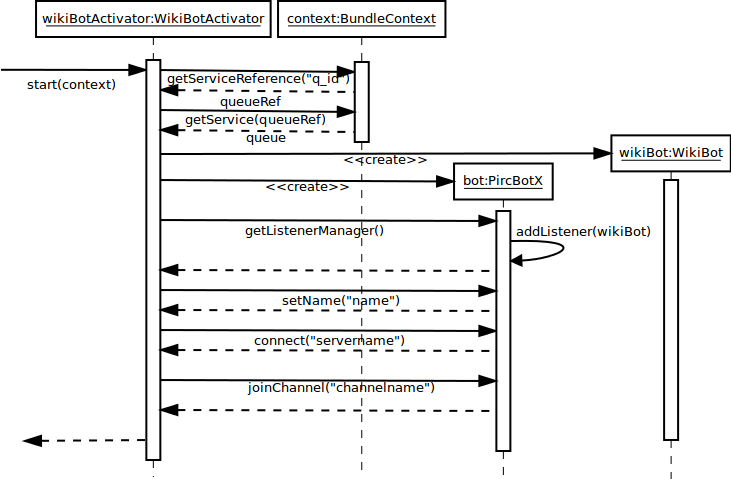
\includegraphics[scale=0.5]{img/sequence_wikiBot}
\caption{WikiBot komponens indulása}
\label{fig:sequence_wikiBot}
\end{figure}

A komponens működése látható a \ref{fig:sequence_wikiBot}.~ábrán: először el kell kérni a QueueManager referenciáját, majd egy PircBotX példányhoz hozzá kell adni egy Listener-t, amely implementálja az eseménykezelőt függvényeket. Ezután meg kell adni az IRCBot nevét, csatlakozni kell egy szerverhez, végül be kell lépni egy IRC csatornába. Ettől a ponttól kezdve, ha egy üzenet érkezik a csatornába (\ref{fig:sequence_wikiBot2}.~ábra), a WikiBot kiszedi a szükséges információkat reguláris kifejezésekkel és elhelyezi a QueueManager-ben.

\begin{figure}[htp]
\centering
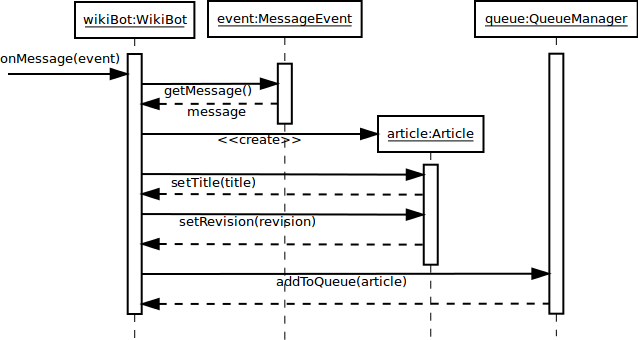
\includegraphics[scale=0.5]{img/sequence_wikiBot2}
\caption{Eseménykezelés a WikiBot-ban}
\label{fig:sequence_wikiBot2}
\end{figure}

% section wikibotbundle (end)

\section{Parser bundle}
\label{sec:parserbundle}

Az összes komponens közül a Parser felépítése a legösszetettebb, többszálú működése miatt egyszerre történik sok minden, ezért a működésen keresztül fogom bemutatni, hogy teljesíti a Parser a tervezésben meghatározottakat.

A komponens indulásakor először megszerzi a kiajánlott adatbázis szolgáltatás referenciáját, a feldolgozás után itt fogja eltárolni a feldolgozott cikkeket azok adataival. Létrehoz ezenkívül egy QueueManager-t, beállít (.addObserver() metódus) számára egy újonnan létrehozott megfigyelőt (WikiObserver osztály), és beregisztrálja a queue-t, mint OSGi szolgáltatást. Végül ha elérhető Wikipedia adatbázis mentés (dump), akkor megkezdi annak feldolgozását is. Az indulás folyamata figyelhető meg a \ref{fig:sequence_parser}.~ábrán.

\begin{figure}[htp]
\centering
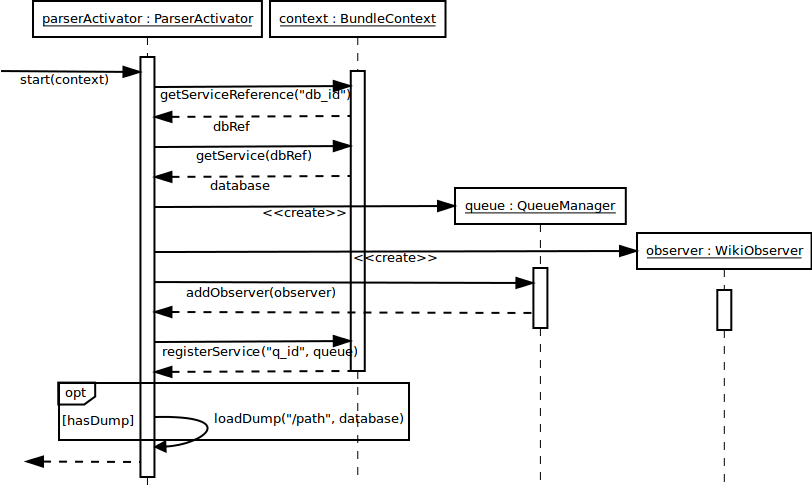
\includegraphics[scale=0.5]{img/sequence_parser}
\caption{A Parser komponens indulása}
\label{fig:sequence_parser}
\end{figure}

A cikkek feldolgozása külön szálakon történik meg, a minél gyorsabb működés érdekében. Minden cikkhez külön Thread objektum példányosítása rendkívül nagy overhead-del járna, ezért a \ref{cha:design} fejezetben már említett ThreadPool mintát használtam. Ez a minta a Thread objektumok újrahasznosításával működik, így nem szükséges mindig új szálat példányosítani. Használata a következő \ref{lst:threadpool}.~kódrészletben figyelhető meg, futtatáskor a szálak nevéből látszik, hogy mindig újrahasználjuk a kezdeti 10 darab szálat:

\begin{lstlisting}[label={lst:threadpool}, caption=ThreadPool használata,breaklines=true]
public class ThreadPoolExample {
    public static void main(String args[]){
       ExecutorService service = Executors.newFixedThreadPool(10);
       for (int i = 0; i < 100; i++){
           service.execute(new Runnable() {
        	   public void run() {
        		    System.out.println(Thread.currentThread().getName());
        			try {
						Thread.sleep(1000);
					} catch (InterruptedException e) {
						e.printStackTrace();
					}
        	   }   
           });
       }
    }
}
\end{lstlisting}

A Parser működése az eddigieket felhasználva a következő:

\begin{figure}[htp]
\centering
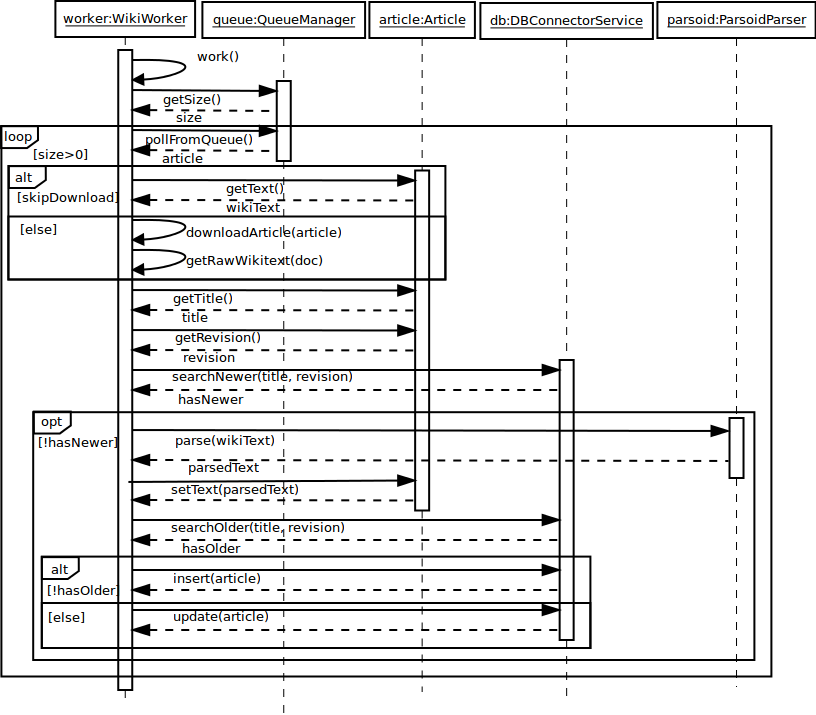
\includegraphics[scale=0.5]{img/sequence_parser2}
\caption{A WikiWorker szál működése}
\label{fig:sequence_parser2}
\end{figure}

\begin{enumerate}
	\item Ha egy új cikk kerül a QueueManager-be, akkor az Observer mintán keresztül a WikiObserver arról értesül.
	\item A WikiObserver egy új WikiWorker szálat rendel a ThreadPool-ból a feladathoz, mely megkezdi a cikk előfeldolgozását (\ref{fig:sequence_parser2}.~ábrán .work() metódus).
	\item A szál addig fut, amíg van feldolgozatlan cikk a queue-ban. A dump feldolgozásban fut a szál, akkor nem kell letölteni a cikkek szövegét, mert azokat ilyenkor a dump-ból már megszereztük. Ellenkező esetben le kell tölteni a hivatalos Wikipedia API-n keresztül a cikket XML formátumban, és ki kell szedni a Wikitext formátumban lévő szövegét.
	\item Ha van az adatbázisban már (.searchNewer() metódus) újabb verziójú cikk az adott cikkből, akkor nem kell tenni semmit, hiszen valószínűleg egy dump feldolgozásban vagyunk és korábban már on-the-fly megszereztük a cikk egy újabb verzióját.
	\item Ha nincs újabb verziójú cikk, akkor a Wikitext formátumról HTML (RDFa) formátumra kell alakítani a szöveget (.parse() metódus).
	\item Ha az adatbázisban van már régebbi verziójú cikk az adott cikkből, akkor valószínűleg on-the-fly feldolgozásban vagyunk és korábban már megszereztük a cikk egy korábbi verzióját. Ekkor az adatbázisban csak frissíteni kell a cikk adatait, máskülönben újonnan kell beilleszteni a cikket.
\end{enumerate}

Az előfeldolgozáskor kapott eredmények meghatározzák a feldolgozólánc használhatóságát, így fontos, hogy a megszerzett cikkek Wikitext formátumú szövegét milyen formában tároljuk. A \ref{cha:design}.~fejezetben láttuk, hogy a feldolgozáskor három cserélhető parser használható a rendszerben, melyek különböző képességekkel bírnak. Ezen parserek a Sztakipedia parser, DumbRegexWikipediaParser és a Parsoid parser. A Sztakipedia parser-nél szükség volt az MTA SZTAKI által készített Java nyelvű könyvtár OSGi komponenssé alakítására.

További felhasználás szempontjából a Parsoid készíti a legjobb kimenetet, azonban egyben a leglassabb is. Ezen lassúság kiküszöbölése miatt különösen jó választás a ThreadPool minta, mert a Parsoid szoftver működése jelentősen függ a bemeneti állományoktól. A parserek összehasonlítása teljesítmény szempontjából a \ref{cha:test}.~fejezetben olvasható. A Parsoid egy NodeJS-ben írt modul, így a feldolgozólánchoz való illesztését egy szerver oldali NodeJS alkalmazással oldottam meg, mely a HTTP POST kérések törzsében küldött Wikitext szöveget HTML / RDFa formátumra tudja alakítani és azt adja vissza a klienseknek. Ezzel a megoldással a feldolgozólánc HTTP-n keresztül kommunikálhat a Parsoid példányokkal, melyek akár külön szervereken is futhatnak (Parsoids komponens a \ref{fig:componentdiagram}.~ábrán).

A dump beolvasása szintén ebben a komponensben van implementálva. A Parser indulásakor, ha van elérhető dump file, akkor megkezdi a dump beolvasását. Ezt a folyamatot a DumpLoader osztály vezérli, két nagyobb fázisban történik meg a dump beolvasása. A Wikipedia dump-hoz hasonló méretű, óriás XML adatok olvasása semmiképpen nem történhet olyan eszközzel, amiben a teljes adat reprezentációját egyszerre kell tárolni, mint például a DOM Parser. Az én választásom egy állapotgép alapú megoldás lett, a SAX (Simple API for XML) Parser. A feldolgozás első fázisában a tényleges folyamat nyomonkövethetősége érdekében a DumpPreprocessor megszámolja a dump-ban lévő cikkek (page csomópontok) számát. A DumpReader pedig végigolvassa a dumpot, és ha beolvasott egy teljes cikket, azt beilleszti egy QueueManager-be. Innentől a feldolgozás megegyezik a főszálon történő folyamattal.

% section parserbundle (end)

\section{DatabaseConnector bundle}
\label{sec:dbconnectorbundle}

Ez a komponens a tervezésnek megfelelően elfedi az adatbáziskezelést a többi komponensek elől úgy, hogy felhasználja a kiválasztott H2DB adatbázis JDBC API-ját. A DBConnector komponens indulásakor először az adatbázis állapotát kell ellenőrizni és szükség szerint olyan állapotba kell hozni, hogy a feldolgozólánc dolgozni tudjon vele. Első lépésben csatlakozni kell a H2DB-hez, majd létre kell hozni hozzá egy adatbázisfelhasználót, egy adatbázist, valamint a szükséges táblákat. Ezzel az adatbázis készen áll a feldolgozólánccal való kommunikációra.

A feldolgozásra kerülő rendkívül nagy adatmennyiség miatt érdemes megfontolni indexek létrehozását is az adatbázisban az Articles táblán. Egy ilyen nagy teljesítményű rendszernél számolni kell az indexhasználat hátrányaival is, ugyanis ha több az írások száma, mint az olvasások száma, az indexek készítése jelentős overhead-et jelenthet az adatbázis számára. Az alkalmazás fő célja, hogy adatokat lehessen kiolvasni belőle, ezért elsődlegesen nem az írások, hanem az olvasások sebességét kell megnövelni. Másrészt az alkalmazás logikája is megköveteli, hogy az olvasás gyors legyen, hiszen ahhoz, hogy egy cikket beillesszünk mindenképpen meg kell nézni, hogy az adott cikk szerepel-e már az adatbázisban. A legtöbbet használt attríbútum olvasáskor a cikk címe, így azon hoztam létre indexeket a H2DB-ben.

% section dbconnectorbundle (end)

\section{Logger bundle}
\label{sec:loggerbundle}

A tervezés részben meghatározott funkcióknak megfelelő módon implementáltam a komponenst. Nem kezdtem saját naplózási rendszer kidolgozásába, hanem a már kiforott Apache log4j megoldást építettem be a komponensbe. Az Apache log4j előnyei, hogy a tervezésénél ügyeltek arra, hogy ne legyen túl nagy hatással az instrumentált kód működésére, és ne kelljen az alkalmazást újrafordítani a naplózás beállításainak módosításához. A log4j beállításait egy konfigurációs fájlban tárolja, ahol széleskörű beállítási lehetőségek használatára van mód.

\begin{figure}[htp]
\centering
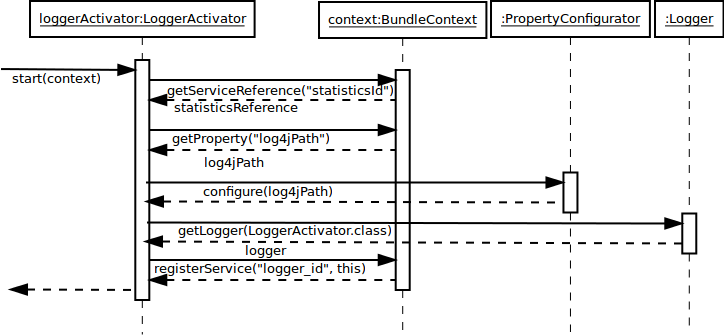
\includegraphics[scale=0.5]{img/sequence_logger}
\caption{A Logger komponens indulása}
\label{fig:sequence_logger}
\end{figure}

OSGi környezetben nem ilyen egyszerű az Apache log4j használata. Alapértelmezett esetben a log4j konfigurációs fájlját (log4j.properties) az alkalmazás gyökérkönyvtárába kell helyezni, OSGi környezetben nyilvánvaló módon ez nem működik. A legegyszerűbb megoldás fragment bundle készítése lenne, melynek nincs BundleActivator osztálya és megosztja classloaderét egy szülő komponenssel. Ennek azonban nagy hátránya van és az Apache log4j egyik előnyét veszítenénk el, mert fragment bundle készítésénél a konfigurációs fájlt a forráskóddal együtt be kellene csomagolni a komponensbe. Így nem lesz konfigurálható a naplózás formája, szintjei, be lesz égetve egy bundle-be minden beállítás.

A fenti hátrányokat elkerülhetjük, ha runtime property-ként megadjuk a helyét a merevlemezen tárolt log4j.properties fájlnak a Felix konfigurációjában. A naplózás beállítását egy szöveges fájlban leírhatjuk és azt a rendszerben bárhol elhelyezhetjük. Az Apache log4j beállítását és OSGi szolgáltatásként való kiajánlását a komponens indulásakor kell megtennünk (\ref{fig:sequence_logger}.~ábra).

% section loggerbundle (end)

\section{Statistics bundle}
\label{sec:statisticsbundle}

A Statistics komponens implementálásakor tehát két servletet és egy adatokat gyüjtő és tárolót kellett létrehozni. A tároló felépítése nagyon egyszerű, a tervezéskor meghatározott metrikákat reprezentáló adatokat tárolja attribútumokban, és implementálja egy kiajánlott OSGi szolgáltatás által meghatározott metrikák módosítására és lekérdezésére szolgáló metódusokat.

A servletek készítése egy kicsit bonyolultabb volt, mert ahhoz, hogy a servlet HTTP-n keresztül elérhető legyen be kell regisztrálni egy servlet container-be. A JEE/J2EE fejlesztés során megszokott web.xml fájlon keresztüli konfigurációt nem használhatjuk, OSGi környezetben, ezért az org.osgi.util.tracker.ServiceTracker osztályban kell beregisztrálnunk servletünket. Ehhez az előbbi osztályból kellett leszármaztatni egy osztályt (HttpServiceTracker a \ref{fig:class_statistics}.~ábrán) és felülírni az addingService és removedService metódusait, ahol be kellett regisztrálni a servlet osztályokat.

\begin{lstlisting}[label={lst:apidata}, caption=A WikiprocessorAPI által szolgáltatott adatok,breaklines=true]
{"articlesData":{"eltárolt cikkek száma":2785,"frissített cikkek száma":877,"újonnan beillesztett cikkek száma":1908,"nem feldolgozott cikkek száma":13},
"logsData":{"error üzenetek száma":3,"warning üzenetek száma":11,"debug üzenetek száma":4},
"queuelength":6013,"mainworkingparsoids":0.5714285714285714,"dumpworkingparsoids":0.8,"dumpprocess":0.11469880217730487}
\end{lstlisting}

A WikiprocessorAPI servlet a metrikák alapján JSON formátumban teszi közzé a feldolgozólánc adatait, így ez a servlet gyakorlatilag egy webes API-nak tekinthető. A StatisticsView egy statikus HTML oldalt szolgál ki, ahol az előbbi API-t felhasználva JavaScript segítségével diagramokat rajzol ki a servlet. A létrehozott diagramok a metrikákat alakítják a felhasználók számára sokkal jobban megfigyelhető formába.

% section statisticsbundle (end)

% chapter implementation (end)
\chapter{Tesztelés és mérések}
\label{cha:test}

\section{A teszteléshez használt eszközök}
\label{sec:testtools}

A feldolgozólánc teszteléséhez elő kellett állítani először a komponensek futtatható változatát. A komponensek implementációjakor használt Bndtools eszköz ebben is nagy segítségemre volt, mert futtatáskor a Bndtools automatikusan előállította a telepíthető csomagokat. Az egyes komponensek könyvtári függőségeit, amelyek nem részei az alap OSGi futtató környezetnek (tipikusan ezek a harmadik féltől származó könyvtárak) magamnak kellett előállítanom szintén a Bndtools segítségével.

A fordításnál előállított JAR formátumú bundle-ök módosítás nélkül telepíthetőek valamilyen OSGi alapú rendszert futtatni képes környezetbe (bundle repository-ba). Fejlesztés során a gyorsabb tesztelhetőség miatt az Eclipse saját OSGi implementációs megoldását az Equinox-ot használtam. Egy stabil változat elkészítése után pedig, bizonyos szinten automatizáltan, szkriptek segítségével telepítettem az alkalmazást a SZTAKI Cloud-ban foglalt virtuális gépre, melyet az alkalmazás futtatására készítettem elő tesztelés céljából.

A telepítési környezetben már a könnyen kezelhető Apache Felix \cite{apachefelix} OSGi implementációját használtam, mert annak WebConsole eszközével könnyedén kezelhetőek a komponensek menedzselése, valamint parancssoros hozzáférés is lehetséges, ahol interaktív módon menedzselhetőek a komponensek, sőt még egy egyszerűbb Bash szintaktikáját utánzó szkriptelési lehetőséget is használhatnak a fejlesztők. Teszteléskor a virtuális gépre SSH-n belépve, az Apache Felix konzolos felületét használva telepítettem az elkészített bundle-öket és függőségeiket.

\begin{figure}[htp]
\centering
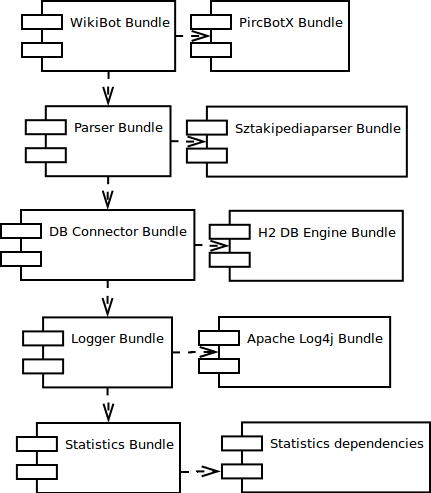
\includegraphics[scale=0.4]{img/deploymentdependency}
\caption{Komponensek függőségei}
\label{fig:deploymentdependency}
\end{figure}

Telepítéshez, illetve a feldolgozólánc komponenseinek frissítéséhez az Apache Felix egy beépített megoldását az Apache Felix Gogo-t használtam, mely egy egységes, szabványos shell felületet határoz meg az OSGi alapú környezetek számára. Amint már említettem az Apache Felix Gogo-val a Unix rendszerekben ismert Bash szintaktikához hasonló parancsokat lehet használni. Ezeket a parancsokat akár szkript formájában is futtathatjuk, ez a Gogo Shell szkript, másnéven \textit{gosh} szkript.

A csomagok függőségeit ábrázolja a \ref{fig:deploymentdependency}.~ábra. A függőségi fa leveleiben található bundle-öket kell először, majd a fában a gyökér felé visszafelé haladva kell a többi bundle-t telepíteni.

A bundle-ök menedzselését a konzolos Apache Felix Gogo Shell-en kívül, egy webes felületen Apache Felix Web Console segítségével is lehet végezni. Segítségével a rendszer állapotát, tulajdonságait lehet beállítani és megfigyelni, valamint a bundle-ök részletes tulajdonságait, kapcsolatait lehet felderíteni, illetve beállításait módosítani. A webes felületről a bundle-ök telepítésével, indításával kapcsolatos funkciók szintén elérhetőek.

% section testtools (end)

\section{A feldolgozóláncra épülő kutatómodul}
\label{sec:researchbundle}

A tesztelés során egy lehetséges felhasználási módot próbáltam ki, mikor a feldolgozólánchoz egy MTA SZTAKI által készített kutatómodult illesztettem. A modul segítségével gépi tanulás, természetes nyelvi feldolgozás témakörökhöz használható program készíthető.

A kutatómodul a feldolgozólánc által készített adatbázisból szerzi meg a bemenő adatokat, ehhez a DB Connector komponens kiegészítése volt szükséges, az OSGi szolgáltatást a lekérdezésekhez szükséges metódussal kellett ellátni. A lekérdezett cikk szövegét, melyet a Parsoid parser HTML / RDFa formátumra alakított, először szintaktikailag helyes XML formátumba kell hozni (valid XHTML).

A kutatómodul a Wikipedia eltárolt cikkeiből ún. AnnotatedDocument példányokat tud készíteni, melyekben a különböző HTML elemek kategóriák szerint vannak már csoportosítva (például: linkek, paragrafusok). Az elkészített gyűjtemények alapján OpenNLP segítségével olyan természetes nyelvi feldolgozáshoz kapcsolódó feladatok végezhetőek, mint például a mondatokra bontás, szóelemzés, tokenizálás.

A kutatómodul végső felhasználása lehet például egy adott kifejezés hivatkozásainak összegyűjtése, hogy milyen kontextusban fordulnak elő a leggyakrabban, meghatározható egy nyelv átlagos szava, vagy bekezdése, rengeteg lehetőség elképzelhető.

% section researchbundle (end)

\section{Mérési eredmények}
\label{sec:measurement}

% TODO

% section measurement (end)

% chapter test (end)
\chapter{Értékelés, továbbfejlesztési lehetőségek}
\label{cha:ending}

A tesztelés és a mérések során arra jutottam, hogy az elkészített feldolgozólánc képes ellátni azokat a feladatokat, és teljesíti a meghatározott követelményeket, melyek a rendszer tervezése előtt célul lettek kitűzve. Az elkészített alkalmazás úgy lett megtervezve, hogy a korábbi megoldások hiányosságait próbálja pótolni és az on-the-fly feldolgozás miatt hiánypótló is lehet a szemistruktúrált adatforrást feldolgozó rendszerek között.

A hasonló megoldások vizsgálatánál láttuk, hogy egy Wikipédiához hasonló mennyiségű adathalmaz feldolgozása semmilyen esetben sem triviális, a használható feldolgozáshoz idő és számítási kapacitás szükséges. A teszteléskor rendelkezésemre álló erőforrások elegendőek voltak a funkcionalitás ellenőrzéséhez, de számítási kapacitásuk a használhatóságot nem érte el. Korábbi vizsgálatok azonban azt mutatták, hogy a rendszer lineárisan skálázódik, így több erőforrás alkalmazásával a feldolgozólánc minden előnyét ki lehet használni.

A rendszer az OSGi keretrendszer előnyeit teljes mértékben kihasználja, a különböző feladatot ellátó komponensek, a WikiBot, Parser és a DBConnector csatolása rendkívül kicsi és azok könnyen menedzselhetőek. Felhasználhatóság szempontjából sokat javított a komponensek funkcionalitásán a felügyeletre tervezés implementálása, a Logger és Statistics komponensek elkészítése.

A SZTAKI által készített elemző kódok integrálása a rendszerbe nagyon könnyű feladat volt. Ez is mutatja, hogy a komponensek jól lettek megtervezve, újabb, más funkcionalitással rendelkező komponens integrálása a rendszerbe sem lenne túl nagy feladat. Remélhetőleg más kutató modulok beépítésére is sor kerül a jövőben, és hasznos segítsége lehet a kutatásoknak a WikiProcessor feldolgozólánc. További kiegészítések és továbbfejlesztési lehetőségek lehetőségeit a következő pontokban foglalom össze.

\begin{description}
	\item[Parser komponens hálózati művelet nélkül]

A mérés során láttuk, hogy a rendszer rendkívül sokat vár hálózati kommunikációra. Egy ilyen nagy teljesítményű rendszernél ez hátrányosan befolyásolja a működést, így érdemes lenne a rendszer leglassabb részét a Parsoid parsert beépíteni a feldolgozóláncba, illetve a hálózati kommunikációt minél jobban kikerülni. Ehhez egyrészt a ParsoidWorker-eket a WikiHarvester géppel azonos gépre kell költöztetni, de hálózati kommunikáció megszűntével elért gyorsítás miatt valószínűleg kevesebb példány futtatása is elegendő lenne.

A kommunikáció azonban a NodeJS-ben írt Parsoid és az OSGi platform között nem egyszerű feladat, így több alternatívát is érdemes lesz kipróbálni. A különböző technológiát használó alkalmazások kommunikációjára egy lehetséges megoldás lehet az interprocessz kommunikáció (\textit{IPC}), amelyet mindkét nyelvből natív módon is el lehet érni, például \textit{MessageQueue} használatával. Másik lehetőség lehet a NodeJS C++-ban implementált V8 JavaScript motorja és az OSGi közötti kommunikáció \textit{JNI} segítségével. A NodeJS-hez létezik is már JNI wrapper a Java API-hoz, így a kommunikáció megoldható lenne, ennek a modulnak a segítségével.

    \item[Feldolgozóláncok készítése egyszerűbben, illetve dinamikusan]

Az eredeti feldolgozólánc architektúrája, melyben nem szerepelt még a dumpfeldolgozás, nagyon egyszerű és átlátható volt, így a célnak megfelelt. A jó tervezésnek köszönhetően a dump feldolgozás is csak két meglévő osztály példányosítását és egy a feladatot végző rész implementációját igényelte. Ebben a helyzetben még mindig elég egyszerű és átlátható a rendszer működése, de látható, hogy az ilyen jellegű kiegészítések szempontjából nem skálázódik egy idő után túl jól a rendszer. Újabb feldolgozási láncok kialakítására a jelenlegiek mellett tehát egyre nehezebbé válik. Ennek a problémának a megoldása lehet, ezen feldolgozóláncok létrehozásának általánosítása.
    
Egyik lehetőség lehet az \textit{Apache Stanbol} nyíltforráskódú és moduláris szoftver stack kiegészítése az eddig elkészített feldolgozólánccal, mely az Apache Stanbol részeként használhatná az teljes software stack egyes komponenseit. Az Apache Stanbol szintén Apache Felix-et használ OSGi futtatókörnyezetként, így ilyen szempontból nem lenne bonyolult a megoldás kivitelezése. A feldolgozóláncok dinamikus előállítása a Stanbol-ban elérhető \textit{Enhancement Chain}-ek segítségével válna elérhetővé. Ennek a megoldásnak a hátránya, hogy az Apache Stanbol funkcióit nem egészítené ki a feldolgozólánc, hanem inkább csak használna azokból néhányat.
    
A fent felsorolt okok miatt érdemes lehet, saját implementációt készíteni a feldolgozóláncok készítéséhez, könnyen kiegészíthető és továbbfejleszthető architektúrával. Ilyen problémák megoldására készült az \textit{Apache Commons Chain} implementációja, mely a \textit{Chain of Responsibility} és \textit{Command} tervezési minta kombinációja.
    
A Chain of Responsibility minta alapgondolata az, hogy szétválasztja a kérést küldõket a fogadóktól azáltal, hogy több objektumnak adja meg a lehetõséget a kérés lekezelésére. A kérés egy objektumokból álló lánc láncszemeit járja be egészen addig, amíg valamelyik láncszem le nem kezeli.
    
A Command minta parancsok, kérések objektumba ágyazását, és ezen keresztül feladatok delegálását fogalmazza meg. Különféle parancsokat rendelhetünk így klienseinkhez (akár dinamikusan is), a parancsokokat akár sorba is állíthatjuk, naplózhatjuk, illetve segítségével visszavonható műveleteket kezelhetünk.
    
    \item[Feldolgozólánc perzisztenciája]

A jelenlegi rendszer leállásával a működéssel kapcsolatos több információ is elveszik azokban a komponensekben, melyek működése nem állapotmentes. Az egyik ilyen kiegészítés lehetne, hogy ha már egyszer feldolgozott a rendszer indulás után egy teljes Wikipédia dump-ot, egy következő indításnál nem érdemes még egyszer megtenni azt.

Leállításkor lehetőség van az OSGi komponensekben az aktuális futás közben használt információk elmentésére az adatbázisban. Például a QueueManager példányokban tárolt információkat ilyenkor lehetne elmenteni, vagy a Statistics komponens által készített statisztikák eltárolását is ekkor kellene megoldani.
\end{description}

A félév során folyamatosan újabb és újabb technológiákat ismertem meg, ezekben sikerült kellőképpen elmélyedni, így azt hiszem rengeteget tanultam az elvégzett munka alatt. Ezenkívül sikerült egy olyan szoftverrendszer teljes életciklusát végigkövetni és megvalósítani, mely megfelel a kitűzött céloknak és egy használható keretrendszert nyújt azok számára, akik egy ilyen hatalmas tudásbázist akarnak egyszerűen felhasználni, mint a Wikipédia.

% chapter ending (end)

% Jegyzékek
\listoffigures \addcontentsline{toc}{chapter}{Ábrák jegyzéke}
\listoftables \addcontentsline{toc}{chapter}{Táblázatok jegyzéke}
\lstlistoflistings \addcontentsline{toc}{chapter}{Forráskódok jegyzéke}

% Bibliography
\clearpage
\addcontentsline{toc}{chapter}{Irodalomjegyzék}
\nocite{*}
\bibliographystyle{plain}
\bibliography{/home/chef/Egyetem/Szakdolgozat/thesis/thesis.bib}

% Függelék
%----------------------------------------------------------------------------
\appendix
%----------------------------------------------------------------------------

\chapter*{Függelék}\addcontentsline{toc}{chapter}{Függelék}




\label{page:last}

\end{document}